% \documentclass{article}
% \usepackage[T1]{fontenc}     % Add this line to ensure scalable fonts
% % \usepackage{ragged2e}        % Provides better justification tools
% \usepackage[protrusion=true,expansion=false]{microtype}  % Disable expansion

% % Line numbering package (add early like in the reference document)
% \usepackage{setspace,lineno}

\documentclass[twocolumn]{article}
\usepackage{lmodern} 
\usepackage[T1]{fontenc}
\usepackage{forest}
% Page geometry - adjusted for line numbers
\usepackage{geometry}
%\usepackage{biblatex}
\geometry{
    letterpaper, 
    left=0.5in,  
    right=0.5in, 
    top=0.5in,   
    bottom=0.5in,
    includeheadfoot,
    twoside=false 
}
\setlength{\columnsep}{25pt}

% Line numbering package (add early like in the reference document)
\usepackage{setspace,lineno}

\usepackage{graphicx}
\usepackage{multirow}
\usepackage{caption}
\usepackage{amsmath,amssymb,amsfonts}
\usepackage{mathtools} 
\usepackage{amsthm}
\usepackage{mathrsfs}
\usepackage[title]{appendix}
\usepackage{xcolor}
\usepackage{float}
\usepackage{textcomp}
\usepackage{algorithm}
\usepackage{algpseudocode}  % Using algpseudocode for better formatting
\usepackage{amsmath}
\usepackage{xcolor}
\providecommand{\algorithmicreturn}{\textbf{return}}
\providecommand{\RETURN}{\State \algorithmicreturn}
\usepackage{setspace,lineno}
\usepackage{booktabs}
\usepackage{multicol}
\usepackage{pifont}
\usepackage{cite}
\usepackage{manyfoot}
\usepackage{algorithmicx}
\usepackage{listings}
\usepackage{tablefootnote}
\usepackage[table,xcdraw]{xcolor}

\usepackage{hyperref}
\hypersetup{
    colorlinks=true,
    linkcolor=blue,
    citecolor=blue,
    urlcolor=blue
}

\definecolor{customgreen}{HTML}{00B050}
\newcommand{\cmark}{\textcolor{customgreen}{\ding{51}}} 
\newcommand{\xmark}{\textcolor{red}{\ding{55}}} 
\raggedbottom

\title{Quantitative Measurement of Parkinson Disease Progression Using DaTscan Radiomics and Clinical Features with a Machine Learning Based Approach}

\author{
Md Mahbub Alam\textsuperscript{1}, 
Subhey Sadi Rahman\textsuperscript{1}, 
Sadia Sultana Chowa\textsuperscript{2}, 
Md. Abdur Rahman\textsuperscript{1}, \\
 Md Rafiqul Islam\textsuperscript{3},  
Sami Azam\textsuperscript{3,*}\\
\small
\textsuperscript{1}Department of Computer Science and Engineering, United International University, Dhaka, 1212, Bangladesh \\
\small
\textsuperscript{2}Health Informatics Research Laboratory (HIRL), Daffodil International University, Dhaka, 1341, Bangladesh \\
\small
\textsuperscript{3}Faculty of Science and Technology, Charles Darwin University, Casuarina, NT 0909, Australia \\
\small 
\textsuperscript{*} Corresponding Author: sami.azam@cdu.edu.au
}

\date{} % Leave date blank

\begin{document}
\justifying
\twocolumn[
\maketitle
\begin{abstract}
\noindent Parkinson's disease (PD) is one of the fastest-growing neurodegenerative disorders, where timely diagnosis is essential for optimizing treatment. In this study, we created a Radiomics-MDS-UPDRS, a robust dataset by integrating DaTscan SPECT radiomics data with the clinical characteristics of MDS-UPDRS collected from Parkinson’s Progression Markers Initiative (PPMI) to monitor dopamine depletion in the striatum (caudate and putamen) and allow classification and progression analysis of PD. To construct the dataset, the striatum was segmented using a modified K-Means clustering algorithm, extracting 25 radiomics features combined with 59 clinical features. In addition, linear discriminant analysis was used to select 22 significant characteristics, and a four-way feature selection method was used to identify 30 significant clinical features, resulting in a refined set of 52. Classification with machine learning models improved performance after LDA, achieving over 91\% accuracy. We evaluated feature behavior across six PD severity stages and four clinical visits for progression analysis. The clinical features of MDS-UPDRS were more sensitive to changes in the severity of the initial PD. At the same time, the integrated dataset, Radiomics-MDS-UPDRS, provided more balanced insights, showing a progression of 33.30\% to 83.30\% and 36.36\% to 45.50\% from the first visit to the fourth visit among the clinical and radiomics features and a progression of 73.33\% to 96.67\% and 13.64\% to 54.55\% between the Minimal vs Mild and Minimal vs Very Severe stage. Our analysis also revealed practical links between progression features and real-life scenarios, which highlights the practical value of our study for clinical decision-making.
\end{abstract}

\vspace{0.5em}
\noindent \textbf{Keywords:} Parkinson’s Disease; DaTscan SPECT Imaging; Disease Progression Analysis; Machine Learning; Feature Selection Techniques
\vspace{1em}
]

\linenumbers

\section{Introduction}

\textcolor{blue}{Parkinson's disease (PD) is the second most prevalent neurodegenerative disorder, first described almost two centuries ago, characterized by the progressive death of dopamine-producing brain cells among older adults . Although the actual cause of PD remains unknown, a combination of environmental, genetic, gender, and age-related factors is believed to contribute to its onset \cite{DBLP:journals/fgcs/AbdulhayNNVV18}. PD affects approximately 2–3\% of people 65 years of age and older \cite{lundervold2019overview}, and the clinical progression of Parkinson's disease over time is highly variable, with certain individuals exhibiting a slowly evolving and minimally deteriorating trajectory, while others experience an accelerated decline in motor and functional impairment. This inter-individual and intra-individual variability of PD expression, in turn, is the cause of diagnostic uncertainty, particularly in early-phase presentations. This diversity requires a highly individualized approach to analyze progression.}

\textcolor{blue}{PD predominantly affects dopaminergic neurons in the substantia nigra, which is a specific region of the brain responsible for the production of dopamine. Lack of dopamine in PD leads to motor dysfunction and a variety of symptoms, including bradykinesia, rigidity, tremors, postural imbalance, sleep disorders, and depression, all of which impact speech, coordination, gait, and balance \cite{majhi2024improved}. Currently, various neuroimaging modalities, such as magnetic resonance imaging (MRI), single photon emission computed tomography (SPECT), and positron emission tomography (PET), are used to diagnose PD \cite{hirschauer2015computer, suwijn2015diagnostic, adeli2017kernel, khachnaoui2020machine}. These imaging techniques can detect PD accurately, but they rely on identifying loss of dopaminergic neurons within the substantia nigra. Traditionally, these medical images are interpreted manually, leaving room for possible human error.}

\textcolor{blue}{Previous studies on PD diagnosis have shown promise but exhibit limitations, such as reliance on specific imaging modalities (e.g., fMRI, SPECT, DTI) or clinical data, overlooking PD progression variability. Chen et al. \cite{chen2023detection} aimed to classify PD patients using machine learning models based on diffusion tensor imaging (DTI) with a sample size of 120 PD patients, and achieved a classification accuracy of 91.67\%. Booth et al. \cite{booth2022predicting} focused on predicting the progression using a support vector machine (SVM) algorithm based on fluorodeoxyglucose-PET (FDG-PET) scans. Their training data included only 43 PD-MCI patients and their SVM model gave an accuracy of 73.7\% when evaluated on a testing set of 19 patients. Later, Fiorenzato et al. \cite{fiorenzato2024brain} compared the effectiveness of Higuchi's fractal dimension (FD) and fractional amplitude of low-frequency fluctuations (fALFF) from resting-state fMRI data in 118 PD patients. Using SVM, they achieved an overall accuracy of 78\% in FD-based features, 62.2\% in fALFF features, and 76\% in a combination of both features. On the other hand, Amboni et al. \cite{amboni2022machine} identified features that are associated with PD-MCI and developed an ML algorithm to distinguish between PD patients with and without MCI. Using a cohort of 75 patients, their first model using clinical characteristics and gait features reached an accuracy of 80\%. However, their second model, which combines the top features from the first model and amyloid PET features, achieved a lower accuracy of 72.2\%.}

\textcolor{blue}{One critical problem with these studies \cite{chen2023detection, booth2022predicting, fiorenzato2024brain, amboni2022machine} is the use of a relatively small sample size that can limit the generalizability and robustness of the ML-based models. In addition, many studies emphasized a single data modality, such as DTI metrics, FDG-PET, fMRI of the resting state, or a combination of clinical and gait data. Relying on a single modality might not capture the full depth of cognitive decline in PD. Lastly, although \cite{booth2022predicting} did perform a progression analysis, \cite{chen2023detection, fiorenzato2024brain, amboni2022machine} primarily conducted classification of patients on their cognitive status at a single time point. They did not track the longitudinal progression of cognitive impairment with their patient samples.}

Our study addresses these gaps by integrating DaTscan SPECT (Dopamine Transporter Scan using Single Photon Emission Computed Tomography) radiomics biomarkers with MDS-UPDRS (Movement Disorder Society Unified Parkinson’s Disease Rating Scale) clinical assessments, creating a dataset to capture PD patterns. Here, clinical features capture functional impairments, while DaTscan SPECT radiomics reveal the structural changes in the substantia nigra region. Then, we employed state-of-the-art feature selection methodologies to understand critical biomarkers and clinical variables that robustly differentiate PD patients across visits, while also illustrating features associated with longitudinal progression of disease severity. Additionally, our study makes use of a large cohort of 228 patients, which leads to more robust and generalizable performance. Lastly, a major contribution to our study lies in the longitudinal assessment of Parkinson's disease progression across four sequential clinical evaluations, identifying significant medical radiomics biomarkers and clinical features that evolve with disease advancement.

The main contributions of this research are:
\begin{itemize}
    \item Developed an automated segmentation method using an improved K-Means clustering algorithm to accurately extract the striatum (caudate and putamen) from DaTscan SPECT radiomics.
    \item Twenty-four imaging features that capture intensity, texture, and geometry were extracted, and 22 significant features with LDA were selected to improve PD classification.  
    \item Introduced Radiomics-MDS-UPDRS, a novel dataset that integrates DaTscan SPECT Radiomics biomarkers with MDS-UPDRS clinical assessments for enhanced Parkinson's disease classification and progression analysis.
    \item Identified the most relevant clinical features for progression analysis using a four-way feature selection strategy, including Random Forest, Mutual Information, Fisher Score, and Recursive Feature Elimination.
    \item Conducted an in-depth analysis of Parkinson's disease progression in different severity stages and patient follow-up visits, using ANOVA, Kruskal-Wallis, and T-tests to uncover key patterns in disease progression.
    \item Analyzed the significance of key features of PD in daily life events.
\end{itemize}

The subsequent sections are organized as follows: Section \ref{Literature Review} reviews the relevant literature on computer-aided Parkinson's disease diagnosis. Meanwhile, Section \ref{Methodology} outlines the study's methodology, including pre-processing techniques, feature extraction, dataset generation, and the proposed framework. Section \ref{Result} presents the experimental results obtained by the proposed framework, along with various comparative analyses. The analysis of Parkinson's disease progression is given in Section \ref{PD Progression}. Section \ref{Discussion} follows a comprehensive discussion, and finally, the paper is concluded in Section \ref{Conclusion}.




\section{Literature Review}
\label{Literature Review}

The diagnosis and progression of PD have been significantly advanced through medical imaging data, particularly with techniques such as SPECT and magnetic resonance imaging combined with machine learning models. Several studies have successfully demonstrated the potential of CNNs to extract meaningful features from neuroimaging data to improve diagnostic accuracy and predict disease progression. 

Their efforts have shown substantial progress, as reflected in the studies by Amoroso et al. \cite{amoroso2018complex}, Khachnaoui et al. \cite{khachnaoui2023enhanced}, Shih-Yen et al. \cite{hsu2020classification}, Magesh et al. \cite{magesh2020explainable}, and Jigna et al. \cite{hathaliya2022convolutional}. Amoroso et al. \cite{amoroso2018complex} proposed a method that combined the characteristics of MRI scans with clinical characteristics. They evaluated the classification performance of 169 healthy controls and 374 patients with PD and achieved an accuracy of 93\%. However, clinical features alone resulted in a lower accuracy of 75\%. Based on this, Khachnaoui et al. \cite{khachnaoui2023enhanced} used SPECT images and pre-trained CNN models (EfficientNet B0, MobileNet V2) to automatically diagnose PD. They applied their method on a larger dataset than Amoroso, of 2720 SPECT DaTscan images (1360 PD and 1360 healthy control subjects from the PPMI database), achieving a high accuracy of 98.47\%. Expanding the scope, Shih-Yen et al. \cite{hsu2020classification} used six pre-trained CNN models (AlexNet, GoogleNet, VGG19, ResNet50, ResNet101, and DenseNet) to classify PD across multiple stages using 99mTc-TRODAT-1 SPECT images. They evaluated 1010 images from 202 cases, classifying them into healthy control (HC), early, middle, and late stages of PD based on the Hoehn and Yahr Scale (HYS). DenseNet achieved an accuracy of 85.5\% in a four-class database. In a similar vein, Magesh et al. \cite{magesh2020explainable} applied a TL technique using the VGG16 model on 642 DaTscan images from the PPMI database to classify them as PD or non-PD and achieved an accuracy of 95.2\%. They also used a local interpretable model-agnostic explanation (LIME) to enhance model interpretability. Jigna et al. \cite{hathaliya2022convolutional} focused on classifying PD according to dopamine levels using 1761 SPECT images from the PPMI database. The images were classified into four categories: PD, HC, SWEDD, and GenRegPD, achieving an accuracy of 88.9\%. Reyes et al. \cite{reyes2019lstm} explored deep learning architectures, achieving 83.1\% accuracy with LSTM, CNN-1D, and CNN-LSTM models. On the other hand, Yagis et al. \cite{DBLP:conf/bibm/YagisHC19} used fMRI images to evaluate the performance of state-of-the-art CNN models in classifying PD and achieved a accuracy of 82.8\% with VGG16 and a accuracy of 88.6\% with ResNet50 in MRI slices from approximately 300 patients, while Ali et al. \cite{ali2019multi} and Martinez et al. \cite{martinez2018kinematic} reported 70\% and 64.1\% accuracy with LDA, respectively. Furthermore, Adeli et al. \cite{adeli2018semi} proposed a semi-supervised discriminative classification method, achieving 79.8\% accuracy. 

\begin{table*}[ht!]
    \centering
    \caption{Summary of related work comparing datasets and associated tasks.}
    \label{tfcomp}
    \scriptsize
    \renewcommand{\arraystretch}{1.3}
    \setlength{\tabcolsep}{4pt}
    \resizebox{\textwidth}{!}{%
    \begin{tabular}{
        >{\centering\arraybackslash}m{3cm}    % Study/Reference
        >{\centering\arraybackslash}m{1.6cm}  % Dataset Name
        >{\centering\arraybackslash}m{1cm}    % Avail.
        >{\centering\arraybackslash}m{1.9cm}  % radiomics Features
        >{\centering\arraybackslash}m{2cm}    % Clinical Features
        >{\centering\arraybackslash}m{1.9cm}  % Progression
        >{\centering\arraybackslash}m{2.5cm}  % # Samples
        >{\centering\arraybackslash}m{2.8cm}  % Task
    }
        \hline
        \multirow{2}{*}{\textbf{Study/Reference}} & 
        \multicolumn{2}{c}{\textbf{Dataset/Corpus}} & 
        \multicolumn{4}{c}{\textbf{Features}} & 
        \multirow{2}{*}{\textbf{Task}} \\
        \cmidrule(lr){2-3} \cmidrule(lr){4-7}
        & \textbf{Dataset Name} & \textbf{Avail.} & \textbf{Radiomics Features} & \textbf{Clinical Features} & \textbf{Progression Analysis} & \textbf{Number of Samples} & \\ \hline

        Amoroso et al. \cite{amoroso2018complex} & PPMI & \cmark & \cmark & \xmark & \xmark & 170 (NC) + 374 (PD) & Classification \\ \hline
        Khachnaoui et al. \cite{khachnaoui2023enhanced} & PPMI & \cmark & \cmark & \xmark & \xmark & 2720 (1360 PD + 1360 HC) & Classification \\ \hline
        Shih-Yen et al. \cite{hsu2020classification} & E-DA Hospital, Taiwan & \xmark & \cmark & \xmark & \xmark & 202 Subjects, 1010 images & Classification \\ \hline
        Magesh et al. \cite{magesh2020explainable} & PPMI & \cmark & \cmark & \xmark & \xmark & 642 images & Classification \\ \hline
        Jigna et al. \cite{hathaliya2022convolutional} & PPMI & \cmark & \cmark & \xmark & \xmark & 1761 images & Classification \\ \hline
        Reyes et al. \cite{reyes2019lstm} & Proprietary dataset & \xmark & \xmark & \xmark & \xmark & 94 (HC) + 88 (PD) & Classification \\ \hline
        Yagis et al. \cite{DBLP:conf/bibm/YagisHC19} & PPMI & \cmark & \cmark & \xmark & \xmark & 300 Subjects & Classification \\ \hline
        Ali et al. \cite{ali2019multi} & Proprietary dataset & \xmark & \xmark & \xmark & \xmark & 20 (PD) + 20 (HC) & Classification \\ \hline
        Martinez et al. \cite{martinez2018kinematic} & Proprietary dataset & \xmark & \xmark & \xmark & \xmark & 11 (PD) + 28 (HC) & Classification using Plantar pressure gait \\ \hline
        Adeli et al. \cite{adeli2018semi} & PPMI & \cmark & \cmark & \xmark & \xmark & 374 (PD) + 169 (HC) & Classification \\ \hline
        Prashanth et al. \cite{DBLP:journals/ijmi/PrashanthRMG16} & PPMI & \cmark & \cmark & \xmark & \cmark & 183 (HC) + 401 (PD) & Classification \\ \hline
        Hajianfar et al. \cite{hajianfar2023prediction} & PPMI & \cmark & \cmark & \cmark & \xmark & 264 (LRRK2) + 129 (GBA) & Pathogenic status prediction \\ \hline
        Harvey et al. \cite{harvey2022machine} & PPMI & \cmark & \xmark & \cmark & \cmark & 423 Subjects & Cognitive diagnosis \\ \hline
        Huang et al. \cite{DBLP:journals/tnn/HuangLCFXEQL22} & PPMI & \cmark & \cmark & \xmark & \cmark & 238 Subjects (62 HC + 142 PD + 34 SWEDD) & Classification and Clinical Score prediction \\ \hline
        Prashanth and Roy \cite{prashanth2018early} & PPMI & \cmark & \xmark & Patient Questionnaire & \xmark & 672 subjects, 5704 records & Classification \\ \hline
        Ali et al. \cite{ali2019reliable} & HandPD & \cmark & Handwritten Drawings & \xmark & \xmark & 92 subjects & Classification \\ \hline
        Castillo-Barnes et al. \cite{castillo2018robust} & PPMI & \cmark & \cmark & Biospecimen & \xmark & 194 (HC) + 168 (PD) + 26 (SWEDD) & Classification \\ \hline
        Ahmadi et al. \cite{ahmadi2019towards} & Proprietary dataset & \xmark & \xmark & \xmark & \xmark & 27 (PD) + 57 (HC) & Classification \\ \hline
        Buongiorno et al. \cite{buongiorno2019low} & Proprietary dataset & \xmark & Motor Function Images & \xmark & \xmark & 14 (HC) + 16 (PD) & Classification \\ \hline
        Cavallo et al. \cite{cavallo2019upper} & Proprietary dataset & \xmark & \xmark & \xmark & \xmark & 30 (HC) + 30 (IH) + 30 (PD) & Classification \\ \hline
        Zhang et al. \cite{zhang2023multi} & PPMI & \cmark & \cmark & \xmark & \xmark & 1032 Subjects & Classification \\ \hline
        Zhang, Xi, et al. \cite{DBLP:conf/amia/Zhang00LZW18} & PPMI & \cmark & \cmark & \xmark & \xmark & 596 (PD) + 158 (HC) & Classification \\ \hline
        \textbf{Our proposed dataset} & \textbf{Radiomics-MDS-UPDRS} & \textbf{\cmark} & \textbf{\cmark} & \textbf{\cmark} & \textbf{\cmark} & \textbf{912 (DaTSCAN + MDS-UPDRS) samples of 228 subjects (PD) at BL, 12M, 24M, 48M} & \textbf{Classification, Progression Analysis, Dataset Generation} \\ \hline
    \end{tabular}}
\end{table*}

While CNN-based approaches have shown promising results in using imaging data for the diagnosis of PD, additional methods that combine clinical features, longitudinal data, and advanced machine learning (ML) algorithms have also been explored to further improve diagnostic accuracy and prediction of disease progression. In this regard, Prashanth et al. \cite{DBLP:journals/ijmi/PrashanthRMG16} demonstrated the potential of combining nonmotor, cerebrospinal fluid (CSF), and imaging markers using ML models, achieving 96.40\% accuracy with an SVM classifier in data from 183 healthy controls and 401 patients with PD in the PPMI database. Hajianfar et al. \cite{hajianfar2023prediction} also demonstrated that combining medical information with SPECT-based imaging features and optimal utilization of hybrid machine learning systems (HMLS) can produce an excellent prediction of the presence of pathogenic gene variants in PD patients. Harvey et al. \cite{harvey2022machine} extended this approach by predicting cognitive outcomes over eight years in newly diagnosed PD patients, showing that combining biological and clinical variables produced models slightly better performing than using clinical data alone. Meanwhile, Huang et al. \cite{DBLP:journals/tnn/HuangLCFXEQL22} highlighted the value of longitudinal multimodal data by proposing an adaptive unsupervised feature selection method based on manifold learning for joint classification and clinical score prediction. Other studies compared multiple traditional ML models. Prashanth and Roy \cite{prashanth2018early} achieved more than 95\% precision using patient questionnaires combined with logistic regression, random forests, boosted trees, and SVM. Similarly, Ali et al. \cite{ali2019reliable} employed a cascade learning system with Chi2, AdaBoost, and Linear Discriminant Analysis (LDA), achieving a precision of 76.44\% along with high sensitivity and specificity. Ensemble models have demonstrated mixed performance, with Castillo-Barnes et al. \cite{castillo2018robust} achieving up to 96\% accuracy and Ahmadi et al. \cite{ahmadi2019towards} reaching a mean sensitivity of 53.7\% by integrating seven ensemble models. Buongiorno et al. \cite{buongiorno2019low} focused on gait and tapping data, achieving 89.4\% accuracy using SVM and ANN. Cavallo et al. \cite{cavallo2019upper} utilized wearable inertial devices and ML models to analyze motion tasks, achieving 95\% precision. The potential of graph-based techniques was shown by Zhang et al. \cite{zhang2023multi} and Zhang, Xi, et al. \cite{DBLP:conf/amia/Zhang00LZW18}. Zhang et al. \cite{zhang2023multi} proposed a multilevel sparsity-based graph learning framework (MGNN) for PD prediction, which incorporates a fast graph construction method and works well on smaller datasets. Similarly, Zhang, Xi et al. \cite{DBLP:conf/amia/Zhang00LZW18} introduced a multiview graph convolutional network (MVGCN) that achieved an AUC of 0.9537±0.0587 by processing brain graphs from multiple views in the PPMI database. 



Although prior studies have shown promise in the diagnosis of PD, several limitations have been observed accordingly. First, reliance on specific datasets, such as imaging modalities such as magnetic resonance imaging (MRI) and SPECT, or motor clinical data, can be the cause of overlooking the variability in the progression of PD. Then, while techniques such as LIME have been used for model interpretability, challenges remain to fully understand how deep learning models make decisions, particularly for complex neuroimaging data. This lack of transparency is a significant disadvantage when analyzing the effective progression of PD. This study addresses these gaps by integrating imaging biomarkers derived from DaTscan SPECT radiomics with comprehensive clinical evaluations from MDS-UPDRS. Our Radiomics-MDS-UPDRS dataset can capture various patterns of PD, which are often overlooked because only clinical markers are used. We have used multiple feature selection methods to enhance interpretability and highlight the contribution of each selected feature. Therefore, our approach offers a balanced understanding of PD by combining classification and progression analysis, making it significant compared to existing methods. A comparative summary of the reviewed literature, their datasets, and their corresponding tasks is presented in Table \ref{tfcomp}.




\begin{figure*}[ht!]
    \centering
    \includegraphics[scale=0.07]{workflow.png}
    \caption{Workflow of the proposed framework.}
    \label{fig:fig1}
\end{figure*}
% ---------------------------------------------
\section{Methodology}
\label{Methodology}

The study is divided into four phases: (1) patient selection and data extraction from the PPMI dataset, (2) data collection, including DaTscan segmentation and feature extraction to create a robust dataset, (3) classification and dimensionality reduction, and (4) feature selection and statistical analysis to evaluate disease progression and significance of features. Figure \ref{fig:fig1} provides an overview of our proposed methodology for the analysis of Parkinson's disease progression. 
% \begin{figure*}
%     \centering
%     \includegraphics[scale=0.09]{Main Diagram.pdf}
%     \caption{Workflow of the proposed framework.}
%     \label{fig:fig1}
% \end{figure*}

% \begin{figure*}
%     \centering
%     \includegraphics[scale=0.25]{overview.png}
%     \caption{Workflow of the proposed framework.}
%     \label{fig:fig1}
% \end{figure*}

% ---------------------------------------------


\subsection{Radiomics-MDS-UPDRS Dataset description}

In this study, we use Parkinson's Progression Markers Initiative (PPMI) \cite{marek2011parkinson} repository to advance the study of biological markers of PD and their progression. The PPMI dataset is divided into three main collections: PPMI Clinical, PPMI Remote, and PPMI Online. 

In this study, we used data from the clinical collection of PPMI, focusing on motor evaluations (MDS-UPDRS) and DaTscan SPECT radiomics. Prior to working with the MDS-UPDRS clinical dataset, appropriate permissions were obtained from the International Parkinson and Movement Disorder Society (MDS). The MDS-UPDRS data we used are categorized into four distinct groups: (1) MDS-UPDRS Part I Patient Questionnaire includes: (i) Cognitive Impairment (NP1COG), (ii) Apathy (NP1APAT); (2) MDS-UPDRS Part I Non-motor Aspects of Daily Living includes: (i) Constipation (NP1CNST), (ii) Fatigue (NP1FATG); (3) MDS-UPDRS Part II Patient Questionnaire: Motor aspects of daily living includes: (i) Eating Tasks (NP2EAT), (ii) Dressing (NP2DRES); and (4) determination of MDS-UPDRS Part III treatment and motor examination includes:

(i) Facial Expression  (NP3FACXP), (ii) Gait (NP3GAIT). 

\textcolor{blue}{For this study, to construct our multimodal Radiomics-MDS-UPDRS dataset, we selected 228 patients with PD from the PPMI clinical dataset. This specific number of patients were chosen because at the time of our experiments their records included a complete and comprehensive set of motor assessments, as well as the corresponding DaTSCAN SPECT imaging data at four longitudinal visits: Baseline, 12, 24 and 48 Months producing 912 imaging studies with synchronized clinical data.} The base MDS-UPDRS dataset, as of April 3, 2024, contained 2,722 unique patient samples distributed as follows: Prodromal (1,233), Parkinson's disease (1,227), Healthy Control (249), non-PD/non-prodromal/non-HC (10), and SWEDD (3). The clinical categories selected from the MDS-UPDRS dataset are presented in Table \ref{tab:tab1}.


\begin{table*}[h]
    \centering
    \caption{MDS-UPDRS clinical data information}
    \label{tab:tab1}
    \small
    \renewcommand{\arraystretch}{1.3} 
    \begin{tabular}{p{5cm}|p{12.5cm}}
    \hline
    \textbf{Category} & \textbf{Features} \\ \hline
    MDS-UPDRS Part I Patient Questionnaire & 
    NP1COG, NP1HALL, NP1DPRS, NP1ANXS, NP1APAT, NP1DDS \\ \hline
    MDS-UPDRS Part I Non-motor Aspects of Daily Living & 
    NP1CNST, NP1FATG, NP1LTHD, NP1PAIN, NP1SLPD, NP1SLPN, NP1URIN \\ \hline
    MDS-UPDRS Part II Patient Questionnaire: Motor Aspects of Daily Living & 
    NP2DRES, NP2EAT, NP2FREZ, NP2HOBB, NP2HWRT, NP2HYGN, NP2RISE, NP2SALV, NP2SPCH, NP2SWAL, NP2TRMR, NP2TURN, NP2WALK \\ \hline
    MDS-UPDRS Part III: Treatment Determination, and Part III: Motor Examination & 
    NP3BRADY, NP3FACXP, NP3FRZGT, NP3FTAPL, NP3FTAPR, NP3GAIT, NP3HMOVL, NP3HMOVR, NP3KTRML, NP3KTRMR, NP3LGAGL, NP3LGAGR, NP3POSTR, NP3PRSPL, NP3PRSPR, NP3PSTBL, NP3PTRML, NP3PTRMR, NP3RIGLL, NP3RIGLU, NP3RIGN, NP3RIGRL, NP3RIGRU, NP3RISNG, NP3RTALJ, NP3RTALL, NP3RTALU, NP3RTARL, NP3RTARU, NP3RTCON, NP3SPCH, NP3TTAPL, NP3TTAPR \\ \hline
    \end{tabular}
\end{table*}

\begin{figure*}
    \centering
    \includegraphics[scale= 0.5]{DatScan.png}
    \caption{DaTscan SPECT with putamen and caudate regions and its segmented view: The left panel shows the original grayscale DICOM image, while the middle panel displays the corresponding heatmap that highlights the region of interest (ROIs) with higher intensity values. The right portion presents the segmented image, where the brightest regions of the heatmap, corresponding to the ROIs, are isolated and highlighted in white against a black background.}
    \label{fig:fig2}
\end{figure*}

\subsection{Putamen and Caudate region segmentation}
The segmentation process starts with isolating specific ROIs from DaTscan SPECT DICOM slices, focusing on three specific slices of 37, 38, and 39. In the dataset, each DICOM slice is accompanied by its corresponding heatmap, which highlights the ROIs. The segmentation process combined both the original image and the heatmap to improve accuracy using K-Means clustering. After converting the DICOM slice into a numerical array, the K-Means algorithm partitions the pixels into a predefined number of clusters. The cluster with the highest brightness is identified as ROI, and all other clusters are suppressed by setting their intensities to zero, preserving only the brightest cluster intact. The resulting segmented image is transformed into grayscale for clarity, with non-zero intensities set to 255 to enhance contrast. This segmentation process effectively highlights ROI, allowing for further analysis depicted in Figure \ref{fig:fig2}. The details of the segmentation algorithm are outlined in Algorithm \ref{algo1}.

\subsubsection{Validation of K-Means Clustering for Segmentation}
\textcolor{blue}{
To validate the robustness of K-Means for striatal segmentation, we conducted a quantitative comparison against three alternative unsupervised clustering algorithms: Gaussian Mixture Model (GMM), Density-Based Spatial Clustering of Applications with Noise (DBSCAN), and MeanShift. Given the inherent challenges in obtaining annotated striatal boundaries for SPECT imaging, we employed three established unsupervised clustering quality metrics: Silhouette Score (cluster separation), Davies-Bouldin Index (cluster compactness), and Calinski-Harabasz Score (variance ratio), as presented in Table \ref{tab:segmentation_comparison}.
}

\begin{table}[ht!]
\centering
\caption{Comparison of algorithms for DaTscan segmentation. Each value represents the mean $\pm$ standard deviation.}
\label{tab:segmentation_comparison}

\fontsize{9pt}{10pt}\selectfont
\renewcommand{\arraystretch}{1}
\setlength{\tabcolsep}{3pt}

\resizebox{\columnwidth}{!}{ % ensures it fits in one column
\begin{tabular}{l c c c c c}
\toprule
\textbf{Algorithm} & 
\textbf{Execution Time (s)} & 
\textbf{Silhouette Score} & 
\textbf{Davies--Bouldin Index} & 
\textbf{Calinski--Harabasz Score} & 
 \\ 
\midrule
K-Means     & \textbf{0.777 $\pm$ 0.018} & \textbf{0.668 $\pm$ 0.039} & \textbf{0.488 $\pm$ 0.053} & 27{,}220 $\pm$ 8{,}362  \\ 
GMM         & 1.922 $\pm$ 0.391 & 0.440 $\pm$ 0.043 & 4.853 $\pm$ 5.745 & 14{,}520 $\pm$ 4{,}759  \\ 
DBSCAN      & 5.681 $\pm$ 1.061 & 0.561 $\pm$ 0.230 & 0.790 $\pm$ 0.634 & 12{,}512 $\pm$ 7{,}768  \\ 
MeanShift   & 0.879 $\pm$ 0.064 & 0.659 $\pm$ 0.037 & 0.554 $\pm$ 0.090 & \textbf{42{,}498 $\pm$ 10{,}180}  \\ 
\bottomrule
\end{tabular}
} % end resizebox
\end{table}
\textcolor{blue}{
K-Means demonstrated superior clustering performance, achieving the highest Silhouette Score (0.668±0.039) and lowest Davies-Bouldin Index (0.488±0.053), indicating optimal cluster separation and compactness. Although MeanShift yielded a higher Calinski-Harabasz score (42,498±10,180), it underperformed on the other two critical metrics. Furthermore, K-Means exhibited consistent results with minimal variability while maintaining computational efficiency (0.777±0.018s). These quantitative results validate K-Means as the optimal segmentation algorithm for this study.
}






% In Figure \ref{fig:fig2}, the left panel shows the original grayscale DICOM radiomics, while the middle panel displays the corresponding heatmap that highlights ROIs with higher intensity values. The right portion presents the segmented radiomics, where the brightest regions of the heatmap, corresponding to the ROIs, are isolated and highlighted in white against a black background.

% ---------------------------------------------
\subsection{Radiomics Feature extraction from Segmented DaTscan SPECT Images}

\textcolor{blue}{From the segmented slices, we extracted twenty-five features that provided insight into the structure and intensity of the striatum. These features included Area, which quantified the size of the segmented region, and the Perimeter-to-Area (PA) ratio, indicating structural elongation defined as Major-Axis length divided by Minor-Axis length. Solidity measured compactness by comparing the area of the segmented region with its convex hull area, which helps to evaluate the integrity of the structure of the striatum. Circularity is assessed by comparing the regularity of the shape with that of a perfect circle. Convex Area is the area of the convex hull enclosing the ROI. Additional geometric features included the Equivalent Diameter, representing the diameter of an equivalent circular region as the ROI, and Extent, a measure of compactness relative to the bounding box of the segmented area. Intensity-based features, including the Mean Intensity and Standard Deviation, captured the average pixel intensity and its variability within the region, reflecting potential changes in dopamine transporter activity. Higher-order statistical features, such as Skewness and Kurtosis, described the asymmetry and peakedness of the intensity distribution. To capture texture, we computed features such as Local Binary Pattern (LBP) Energy and Entropy, as well as Gabor Energy and Entropy, which analyzed the uniformity and complexity of texture patterns. The features derived from the gray-level co-occurrence matrix (GLCM), including Contrast, Homogeneity, Dissimilarity, Correlation, and Energy, revealed relationships between neighboring pixel intensities. Lastly, structural features such as the Lengths of the Major and Minor Axes and the Filled Area offered additional perspectives on the morphology and integrity of the striatum. Major-Axis Length represents the longest principal axis and Minor-Axis Length represents the shortest principal axis of the segmented area's best-fit ellipse.}

\textcolor{blue}{These radiomic features quantify how dopaminergic loss reshapes and redistributes striatal DaT uptake in PD degeneration. Area, Convex Area, Filled Area, Equivalent Diameter, Extent, Circularity, Solidity, and the Major/Minor axis lengths with their PA ratio together reflect whether the normal elongated “comma-shaped” uptake is preserved or has contracted into a smaller, fragmented, more dot-like focus \cite{morbelli2020eanm, mercer2024practical}. Lower Mean intensity indicates reduced dopamine transporter availability, while higher Standard Deviation, Skewness, and Kurtosis capture increasingly uneven, focal residual uptake as the posterior putamen deteriorates compared with the caudate \cite{mayerhoefer2020introduction}. Increased GLCM Contrast and Dissimilarity combined with reduced Energy and Homogeneity indicate sharper local transitions between relatively spared and degenerated subregions, and a decline in GLCM Correlation denotes loss of coordinated gray-level across neighbors. At higher spatial frequencies, a reduction in LBP Energy and increase in LBP Entropy indicate growing irregularity at micro-texture level. On the other hand, orientation-sensitive Gabor Energy declines and Gabor Entropy increases when the charateristic posterior tail dissipates and striatal texture loses oritentation structure.}

\begin{algorithm} [ht!]
\caption{K-Means Clustering for Radiomics Processing}
\label{algo1}
\begin{algorithmic}[1]
\Procedure{process\_dicom}{dicom\_path, num\_clusters}
    \State \texttt{dicom\_data} $\gets$ \texttt{load\_dicom(dicom\_path)}
    \State \texttt{slices} $\gets$ \texttt{extract\_slices(dicom\_data, [37, 38, 39])}
    \For{each slice in slices}
        \State \texttt{img\_array} $\gets$ \texttt{to\_numpy(slice)}
        \State \texttt{pixels} $\gets$ \texttt{reshape(img\_array, (-1, 3))}
        \State $K \gets \text{KMeans}(n\_clusters = \text{num\_clusters}, \text{random\_state}=42)$
        \State $K.\text{fit(pixels)}$
        \State $L \gets K.\text{labels\_}$, \quad $C \gets K.\text{cluster\_centers\_}$
        \State $B \gets \arg\max_j(\sum C[j])$
        \State \texttt{modified\_C} $\gets$ \texttt{zeros\_like(C)}
        \State \texttt{modified\_C[B]} $\gets$ \texttt{C[B]}
        \State \texttt{compressed\_img\_array} $\gets$ \texttt{reshape(modified\_C[L], img\_array.shape)}
        \State \texttt{compressed\_img} $\gets$ \texttt{to\_images(compressed\_img\_array)}
        \State \texttt{slice\_array} $\gets$ \texttt{to\_numpy(compressed\_img)}
        \State \texttt{slice\_array[slice\_array $\neq$ 0]} $\gets$ \texttt{255}
        \State \texttt{modified\_slice\_images} $\gets$ \texttt{to\_images(slice\_array)}
        \State \texttt{grayscale\_images} $\gets$ \texttt{convert\_to\_grayscale(modified\_slice\_images)}
        \State \textbf{save} grayscale\_images to output\_images\_path
    \EndFor
    \State \textbf{Output:} Grayscale segmented ROI images for slices 37--39
\EndProcedure
\end{algorithmic}
\end{algorithm}

% ---------------------------------------------
\subsection{Radiomics-MDS-UPDRS dataset generation}

To analyze the progression of Parkinson’s disease, we selected patients with periodic DaTscan imaging at four time points: baseline, month 12, month 24, and month 48. From a total of 4433 scans, we identified 228 patients who met this criterion, resulting in 912 DaTscans for the study of each patient who had four DaTscans. For each scan, the segmentation and feature extraction process yielded a comprehensive quantitative measure radiomics dataset. After the segmentation and feature extraction from the scans, we took the clinical MDS-UPDRS motor assessment data and four assessment data points for each patient. The clinical assessment data was combined with the extracted radiomics feature data, ensuring alignment based on assessment date, event ID, and patient ID. This integration was performed with meticulous human evaluation to preserve the accuracy of the data. After combining the two datasets, we were able to construct Radiomics-MDS-UPDRS, a hybrid dataset of 84 features. This combined dataset serves as a foundation for understanding the progression of PD and evaluating its impact on the striatum in different stages.





Feature selection plays a crucial role in the machine learning process, enabling the identification of the most relevant and informative features of a dataset. In this study, we used LDA to select radiomics features from DaTscan SPECT. Additionally, we applied four distinct feature selection techniques: Forest Feature Extraction (RFFE), Mutual Information Score (MI), Fisher Score (FS), and Recursive Feature Elimination (RFE) to identify the most significant clinical features, ensuring a robust and meaningful analysis.


\subsubsection{Linear Discriminant Analysis}

This study used LDA as a dimensionality reduction technique to transfer the high-dimensional feature space into a lower-dimensional space that optimizes class separability. LDA is a supervised method that aims to project the data onto a subspace where the classes are most distinguishable. LDA finds the linear combination of the original feature set that maximizes the ratio of between-class variance to within-class variance, which tries to ensure that the projected data are as spread out as possible between classes while minimizing the spread within each class. The LDA is calculated as shown in Equation \eqref{eq:eq1}:
\begin{equation}
    W = \arg\max_w \frac{W^T S_b W}{W^T S_W W}
    \label{eq:eq1}
\end{equation}

\begin{figure*}
    \centering
    \includegraphics[width=\textwidth]{LDA_Diagram.drawio.png}
    \caption{\textcolor{blue}{Clustering of the LDA components and comparing the clusters with true disease severity levels.}}
    \label{fig3}
\end{figure*}

The main objective is to find a $W$ transformation matrix that maximizes the ratio of the scatter matrix between classes $S_b$ to the scatter matrix within classes $S_W$. Here, $S_W$ is the scatter matrix within the class. $S_W$ captures the variance within each class by summing the covariance of the data points around their respective class mean. The within-class scatter matrix is defined in Equation \eqref{eq:eq2}:
\begin{equation}
    S_W=\sum_{c=1}^{C}\sum_{x_i\epsilon c}(x_i - \mu_c)(x_i - \mu_c)^T
    \label{eq:eq2}
\end{equation}
where $x_i$ is a data point in class $c$, $\mu_c$ is the mean vector of class $c$, and $C$ is the number of classes. $S_B$ is the between-class scatter matrix, which measures the variance between class means, as shown in Equation \eqref{eq:eq3}:
\begin{equation}
    S_B=\sum_{c=1}^{C}n_c(\mu_c - \mu)(\mu_c - \mu)^T
    \label{eq:eq3}
\end{equation}
where $\mu_c$ is the mean vector of class $C$, and $\mu$ is the overall mean vector of the dataset. $n_c$ is the number of samples in class $C$. Once the means of the class and the scatter matrix are calculated, the next step in LDA involves finding the eigenvectors and eigenvalues of the matrix $S_W^{-1}S_B$. These eigenvectors, as defined in Equation \eqref{eq:eq4}, represent the direction in the feature space along with the data that show the greatest separation between classes.
\begin{equation}
    S_W^{-1}S_Bw = \lambda w
    \label{eq:eq4}
\end{equation}
In Equation \eqref{eq:eq4}, $w$ is the matrix of eigenvectors (the LDA coefficients or scalings), and $\lambda$ is the diagonal matrix of eigenvalues. The eigenvectors derived from this eigenvalue problem represent the optimal projection directions that maximize class separability.

We transfer the higher-dimensional dataset with 84 features to 2 linear discriminants, which cover the 96\% variance of the total dataset. After transforming the higher-dimensional dataset into the lower-dimensional dataset, we cluster the linear discriminant (LD) using Agglomerative clustering and K-means clustering techniques to ensure that the LDs properly create distinct clusters among different severity levels (see Figure \ref{fig3}).

\subsection{Feature selection}
% ---------------------------------------------
\subsubsection{Random Forest feature extraction}

RFFE is a technique that uses a random forest algorithm, which is an ensemble learning method that combines multiple decision trees to make a more accurate model to assess the importance of each feature. Feature importance in Random Forests is measured by how much each feature decreases the impurity (e.g., Gini impurity or entropy) across all the trees in the forest. The Gini Impurity for a node is calculated as shown in Equation \eqref{eq:eq5}:
\begin{equation}
    Gini_i = 1 - \sum_{k=1}^{C}P_k^2
    \label{eq:eq5}
\end{equation}

The feature importance $FI$ of feature j is the average decrease in Gini impurity across all trees $T$ in the forest, which is calculated as shown in Equation \eqref{eq:eq6}:
\begin{equation}
    FI(x_j) = \frac{1}{T}\sum_{t-1}^{T}\sum_{n\epsilon N(f,t)}(Gini_{before} - Gini_{after})_n
    \label{eq:eq6}
\end{equation}

where $FI$ is the feature importance $T$ is the total number of trees in the Random Forest, $N(f,t)$ is the set of all nodes in the tree $t$ where $f$ is the features used for splitting.

In our study, we used RFFE to pinpoint the key clinical and imaging features. This approach helps us reduce the feature set of the data while retaining the most important information for accurately assessing disease stages and tracking their progression.

% ---------------------------------------------
\subsubsection{Mutual Information score}

The Mutual Information (MI) score measures how much the feature reduces uncertainty about the target class, and it captures any relationship between features and the class. Features with higher MI scores are considered more important. It quantifies the amount of shared information between a feature and a class. For our case, to stabilize the feature selection, we average the score over multiple runs and select the features with the highest average MI. The Mutual information score is calculated using Equation \eqref{eq:eq7}:
\begin{equation}
    I(X_i, Y) = \sum_{x_i\epsilon X_i}\sum_{y\epsilon Y}p(x_i, y)\log\frac{p(x_i, y)}{p(x_i)p(y)}
    \label{eq:eq7}
\end{equation}

where $p\left(x_i,y\right)$ is the joint probability of $X_i$ and $Y$. $p\left(x_i\right)$ and $p\left(y\right)$ are the marginal probabilities of $X_i$ and $Y$. By using MI for feature extraction, we ensure that the selected features effectively capture the shared information between the data and disease stages.

% ---------------------------------------------
\subsubsection{Fisher Score}

Fisher Score is another feature selection technique that assesses the biased ability of features, based on the class distribution within a dataset. It takes the amount of ratio of the variance among the classes to the variance within classes. Features with a higher Fisher score are more likely to be relevant. Fisher Score is calculated using Equation \eqref{eq:eq8}:
\begin{equation}
    F_i = \frac{\sum_{k=1}^{C}N_k(\mu_{i,k}-\mu_i)^2}{\sum_{k=1}^{C}N_k\sigma_{i,k}^2}
    \label{eq:eq8}
\end{equation}

where $C$ is the number of classes and $N_k$ is the number of samples in class $k$. $\mu_{i,k}$ is the mean of feature  for class $k$. $\mu_i$ is the overall mean of features. $\sigma_{i,k}^2$ is the variance of a feature within class $k$.

In our study, we use the Fisher Score for feature selection to evaluate the discriminative power of clinical and imaging features by examining the variance between classes. This approach helps in identifying the features that best differentiate between Parkinson's disease stages.

% ---------------------------------------------
\subsubsection{Recursive feature elimination}

RFE is a wrapper-type feature selection algorithm. The goal of RFE is to select important features by recursively considering smaller and smaller sets of features, discarding the least important ones, and refitting the model. Features are scored using either an ML model or a statistical method. In our case, we use Logistic regression for feature selection using Recursive feature Elimination. Equation \eqref{eq:eq9} shows the RFE calculation:
\begin{equation}
    y = \frac{1}{1+e^{-(\beta_0 + \sum_{i=1}^n\beta_iX_i)}}
    \label{eq:eq9}
\end{equation}
where $X_i$ is the feature value $\beta_i$ is the coefficient of $X_i$ and $\beta_0$ is the intercept and $y$ is the predicted probability. In RFE features with smaller ${|\beta}_i|$ are eliminated because they contribute less to the prediction of $y$. We use Recursive Feature Elimination (RFE) to identify the most relevant clinical and imaging features by iteratively eliminating less important ones.

In addition to these ML-based feature selections, we also use LDA to select important features. It is a supervised algorithm that is used for dimensionality reduction. Maximizes the variance between classes, minimizes the variance within classes, and projects higher-dimensional data into lower dimensions. In feature selection, it identifies the most important features that maximize the separation between classes. The higher the score, the more important the feature for LDA. Table \ref{tab:tab4} shows that LDA gives priority mainly to the radiomics feature.

% ---------------------------------------------
\subsection{Classification: combined vs. lower dimension dataset}
\textcolor{blue}{The classification was performed on the combined dataset using thirteen machine learning models, comprising eight traditional classifiers (RF, LR, DT, GB, KNN, SVM, NB, XGB) and five ensemble methods (Extra Trees, Bagging, Voting Hard/Soft, Stacking).The dataset was partitioned into training (70\%) and testing (30\%) subsets using stratified random sampling with a fixed random state (random\_state=42) to ensure reproducibility. We evaluated training accuracy, testing accuracy, precision, recall, F1-score, AUC-ROC, and 95\% confidence intervals both before and after applying LDA with n=2 (see Table \ref{tab:tab2}, and Table \ref{tab:tab4}). The classification results in the lower-dimensional space were significantly improved, showing higher testing accuracy, precision, recall, and F1-score.}


% ---------------------------------------------
\subsection{Feature importance analysis}

Feature importance analysis was performed using ANOVA and the Kruskal-Wallis test to validate the significance of each selected feature by analyzing their p-values. ANOVA is a statistical method used to identify differences between the means of more than two groups by calculating the variance ratio between and within groups, making it a widely recognized approach to classifying characteristics. On the other hand, the Kruskal-Wallis test \cite{ali2014kruskal} is a non-parametric alternative to one-way ANOVA, extending the Mann-Whitney U test to compare two or more groups. It is computationally efficient, easy to use, and tests whether the groups have equal medians, providing a p-value of significance. Features with discriminative information are selected, as indicated by p-values close to 0, while non-discriminative features are excluded. The detailed feature selection process is outlined in the results analysis section.

\subsection{Final features and further analysis}
After the feature selection from the four distinct feature selection techniques and LDA, we have a final dataset of 52 features, where 22 imaging features are selected by LDA and 30 clinical features are selected by the four feature selection techniques. With these final 52 features, the assessment of progression analysis of Parkinson's disease is shown in section \ref{PD Progression}.

\subsection{Longitudinal severity progression modeling}
\label{sec:longitudinal_model}

\textcolor{blue}{We created a longitudinal severity prediction model employing bidirectional Long Short-Term Memory (Bi-LSTM) networks with an attention mechanism in order to capture the temporal dynamics of PD progression.  By processing successive patient observations over time, this architecture directly simulates the evolution of the illness trajectory, in contrast to traditional cross-sectional categorization techniques.  Two stacked Bi-LSTM layers with 128 and 64 hidden units, respectively, make up the network architecture. Dropout regularization (rate = 0.3) is used to reduce overfitting.  In order to enable the algorithm to concentrate on clinically significant time points during progression prediction, an attention layer was incorporated to weight temporal features dynamically.  For probabilistic six-class severity classification (Mild, Minimal, Moderate, Moderate to Severe, Severe, Very Severe), the last dense layer uses softmax activation.
228 PD patients with full data from four consecutive assessment time points (V1(baseline), V2, V3, and V4 follow-ups) made up the longitudinal cohort, which produced 912 total observations.  The combined Radiomics-MDS-UPDRS dataset's 84 features were all used as temporal inputs.  Patient-level stratification was used to maintain temporal integrity and avoid data leakage. The cohort was divided into training (70\%, n=640 sequences), validation (15\%, n=137 sequences), and testing (15\%, n=135 sequences) subsets, making that no patient featured in more than one partition.  The Adam optimizer with a categorical cross-entropy loss function was used for model optimization across 50 epochs, with early halting determined by validation results.  Based on patient-specific progression trajectories, this temporal modeling methodology allows prospective prediction of future severity levels, offering a quantitative basis for individualized disease monitoring and therapeutic}

% ---------------------------------------------
\section{Result Analysis}
\label{Result}

\textcolor{blue}{This section presents the results of two separate analyses: classification and progression analysis of PD. Based on the robust Radiomics-MDS-UPDRS dataset, the classification analysis evaluates thirteen machine learning models, including traditional classifiers and advanced ensemble methods, with comprehensive performance metrics (accuracy, precision, recall, F1-score, AUC, and 95\% confidence intervals) to establish methodological rigor. The second analysis focuses on progression, incorporating the clinical characteristics of MDS-UPDRS, the radiomics features of the DaTscan SPECT radiomics, and the combined data proposed in this study. 
} 


% ---------------------------------------------
\subsection{Classification of PD severity }
\textcolor{blue}{The performance of thirteen ML models is evaluated: eight traditional classifiers—Random Forest (RF), Logistic Regression (LR), Decision Tree (DT), Gradient Boosting (GB), K-Nearest Neighbors (KNN), Support Vector Machine (SVM), Naïve Bayes (NB), Extreme Gradient Boosting (XGB) and five ensemble methods Extra Trees, Bagging, Voting (Hard/Soft), and Stacking presented in Section \ref{sec_4.1.1}. All models include AUC and 95\% confidence intervals for robust performance assessment. LDA-based dimensionality reduction is subsequently employed (Section \ref{sec_4.1.2}) to enhance classification accuracy.}

\subsubsection{Performance of ML models without LDA}
\label{sec_4.1.1}
The classification results of ML models, using the DaTscan SPECT radiomics features, are detailed in this section. Table \ref{tab:tab2} presents the results, including training accuracy, testing accuracy, precision, recall, and F1-scores for each model. 

\begin{table}[ht!]
\small
\centering
\fontsize{7pt}{8pt}\selectfont
\renewcommand{\arraystretch}{1}
\caption{Performance of machine learning models with all DaTscan SPECT radiomics features before LDA. \textbf{Tr}, and \textbf{Te} represent the \textbf{Tr}aining, and \textbf{Te}sting performance, respectively.}
\label{tab:tab2}
\setlength{\tabcolsep}{3pt}

\resizebox{\columnwidth}{!}{ % <—— key line
\begin{tabular}{l c c c c c c c}
\toprule
\textbf{Method} & \textbf{Acc (Tr)} & \textbf{Acc (Te)} & \textbf{Prec (Te)} & \textbf{Recall(Te)} & \textbf{F1 (Te)} & \textbf{CI} & \textbf{AUC} \\ 
\midrule
RF  & 1.00  & 0.64  & 0.68  & 0.64  & 0.61  &[0.59 - 0.70] &0.87\\ 
LR  & 0.99  & 0.83  & 0.84  & 0.83  & 0.82  &[0.79 - 0.87] &0.98\\ 
DT  & 1.00  & 0.42  & 0.44  & 0.42  & 0.42  &[0.39 - 0.50] &0.61\\ 
GB  & 1.00  & 0.64  & 0.65  & 0.64  & 0.62  &[0.60 - 0.71] &0.88\\ 
KNN & 0.72  & 0.57  & 0.61  & 0.57  & 0.55  &[0.51 - 0.63] &0.85\\ 
SVM & 0.97  & 0.82  & 0.86  & 0.82  & 0.81  &[0.78 - 0.87] &0.98\\ 
NB  & 0.54  & 0.48  & 0.66  & 0.48  & 0.48  &[0.43 - 0.55] &0.79\\ 
XGB & 1.00  & 0.62  & 0.62  & 0.62  & 0.60  &[0.58 - 0.69] &0.87\\ 
Extra Trees & 1.00  & 0.65  & 0.65  & 0.66  & 0.62  &[0.60 - 0.71] &0.91\\ 
Bagging (DT) & 1.00  & 0.66  & 0.65  & 0.66  & 0.62  &[0.60 - 0.71] &0.88\\ 
Voting (Hard) & 1.00  & 0.68  & 0.70  & 0.68  & 0.65  &[0.61 - 0.73] &N/A\\ 
Voting (Soft) & 1.00  & 0.68  & 0.69  & 0.68  & 0.65  &[0.61 - 0.73] &0.90\\ 
Stacking & 1.00  & 0.70  & 0.70  & 0.70  & 0.68  &[0.65 - 0.76] &0.94\\ 
\bottomrule
\end{tabular}
} 
\end{table}


\textcolor{blue}{
With F1-scores of 0.82 and 0.81 (AUC: 0.98 for both), LR and SVM perform better than the others in Table \ref{tab:tab2}, successfully capturing underlying radiomics patterns.  Results from ensemble methods are competitive: extra trees (0.65 accuracy, 0.91 AUC), voting strategies (0.68 accuracy, 0.90 AUC), and stacking (0.70 accuracy, 0.94 AUC) outperform individual weak learners.  On the other hand, NB (F1: 0.48) and DT (F1: 0.42) perform poorly.  The ensemble approaches show the benefit of combining multiple models to improve robustness; voting strategies reduce overfitting by providing consensus-based predictions, while stacking achieves the highest AUC (0.94) of all methods.By addressing the need for sophisticated approaches beyond traditional single classifier approaches, the thorough evaluation with AUC and 95\% confidence intervals validates model robustness beyond traditional accuracy metrics.  Interestingly, the confidence intervals show model reliability across severity classes; for high-performing models (LR, SVM), the intervals are narrower ([0.78-0.87]), suggesting consistent predictions, while for weaker models, the intervals are wider, suggesting greater uncertainty in classification decisions.
}


\begin{table}[ht!]
    \centering
    \caption{Top priority features from LDA: Extracted features and their scaling values from Linear Discriminant (LD)}
    \label{tab:tab3}
    \fontsize{6.8pt}{10pt}\selectfont 
    \renewcommand{\arraystretch}{1.3} 
    \begin{tabular}
    % {|p{4cm}|p{3cm}|p{4cm}|p{3cm}|}
    {lc|lc}
    \hline
    \textbf{T20 LD1} & \textbf{Scaling} & \textbf{T20 LD2} & \textbf{Scaling} \\ \hline
    Standard Deviation & -13.866 & Area & 122.3075 \\ 
    Contrast & 13.61688 & Filled Area & -118.63 \\ 
    Gabor Entropy & -12.2778 & Homogeneity & 44.79036 \\ 
    Shannon Entropy & -11.0716 & Standard Deviation & -41.9018 \\ 
    Dissimilarity & -10.2457 & Skewness & -35.7697 \\ 
    Skewness & -8.23307 & Shannon Entropy & 30.08729 \\ 
    Homogeneity & -8.00484 & Contrast & 20.99671 \\ 
    Energy & -7.88104 & Energy & -20.3214 \\ 
    Gabor Energy & 6.730667 & Kurtosis & 18.43916 \\ 
    Mean & 6.301926 & Dissimilarity & -13.4105 \\ 
    Brightness & 6.301926 & Gabor Entropy & -8.93315 \\ 
    Area & 5.5528 & LBP Energy & 8.501743 \\ 
    Filled Area & -4.59068 & Mean & 7.296339 \\ 
    Equivalent Diameter & -4.10329 & Brightness & 7.296339 \\ 
    Major Axis Length & 3.709302 & LBP Entropy & 5.47781 \\ 
    Kurtosis & 3.561322 & Correlation & 3.45925 \\ 
    Convex Area & -3.49746 & Equivalent Diameter & -3.39241 \\ 
    Minor Axis Length & 2.912351 & Gabor Energy & 2.822265 \\ 
    Correlation & 2.476936 & Solidity & 1.855058 \\ 
    LBP Entropy & 1.915438 & Convex Area & 1.625698 \\ \hline
    \end{tabular}
\end{table}

\begin{table}[ht!]
\centering
\caption{Machine learning based classification algorithms result after LDA, with LD1 and LD2. \textbf{Tr}, and \textbf{Te} represent the \textbf{Tr}aining, and \textbf{Te}sting performance, respectively.}
\label{tab:tab4}

\fontsize{9pt}{10pt}\selectfont 
\renewcommand{\arraystretch}{1}
\setlength{\tabcolsep}{3pt}

\resizebox{\columnwidth}{!}{ % <—— Resizes to fit column width
\begin{tabular}{l c c c c c c c}
\toprule
\textbf{Method} & \textbf{Acc (Tr)} & \textbf{Acc (Te)} & \textbf{Prec(Te)} & \textbf{Recall(Te)} & \textbf{F1(Te)} & \textbf{CI} & \textbf{AUC}\\ 
\midrule
RF       &1.00 &0.91 &0.92 &0.91 &0.91 &[0.86 - 0.93] &0.96\\ 
LR       &0.96 &0.90 &0.90 &0.90 &0.90 &[0.84 - 0.92] &0.98\\ 
DT       &1.00 &0.90 &0.90 &0.90 &0.90 &[0.80 - 0.88] &0.90\\ 
GB       &1.00 &0.90 &0.90 &0.90 &0.90 &[0.83 - 0.90] &0.98\\ 
KNN      &0.96 &0.92 &0.92 &0.92 &0.92 &[0.86 - 0.93] &0.96\\ 
SVM      &0.96 &0.90 &0.90 &0.90 &0.90 &[0.86 - 0.93] &0.99\\ 
NB       &0.96 &0.90 &0.91 &0.90 &0.90 &[0.85 - 0.92] &0.99\\ 
XGB      &0.99 &0.91 &0.91 &0.90 &0.90 &[0.87 - 0.93] &0.97\\ 
Extra Trees    &1.00 &0.88 &0.89 &0.88 &0.88 &[0.84 - 0.91] &0.98\\ 
Bagging (DT)   &1.00 &0.88 &0.89 &0.88 &0.88 &[0.84 - 0.91] &0.97\\ 
Voting (Hard)  &1.00 &0.90 &0.90 &0.90 &0.90 &[0.86 - 0.93] &N/A\\ 
Voting (Soft)  &1.00 &0.90 &0.90 &0.89 &0.89 &[0.86 - 0.93] &0.97\\ 
Stacking       &1.00 &0.90 &0.91 &0.90 &0.90 &[0.86 - 0.93] &0.98\\ 
\bottomrule
\end{tabular}
} % <—— End resizebox
\end{table}


\begin{figure*}[ht!]
    \centering
    \includegraphics[width=\textwidth]{LDA_Diagram_PDF_LD1_2.drawio.png}
    \caption{\textcolor{blue}{LDs across different disease severity}}
    \label{fig:fig4}
\end{figure*}



% ---------------------------------------------
\subsubsection{Performance of ML models with LDA}
\label{sec_4.1.2}

Two discriminant axes, LD1 and LD2, are used in the LDA-based ML classification. In both cases, 20 features were selected from the total of 84 features based on their contribution to class separation. The twenty significant features with their scaling values for both LD1 and LD2 are presented in Table \ref{tab:tab3}.



From Table \ref{tab:tab3}, LDA with LD1 and LD2 scaling identified the 20 most informative features, each time contributing to disease severity. For LD1, the most significant features included Contrast, followed by Gabor Energy, Mean, Brightness, and Area. Conversely, features such as Convex Area, Equivalent Diameter, Filled Area, Energy, Homogeneity, Standard Deviation, Gabor Entropy, and Skewness exhibited negative scaling values, indicating their lesser relevance to disease progression. Similarly, for LD2, Area showed the highest scaling score, as well as Homogeneity, Shannon Entropy, Contrast, and Kurtosis ranking next. Additionally, our experiment highlighted the greater importance of DaTscan SPECT radiomics features compared to MDS-UPDRS clinical data, as 20 out of the 24 radiomics-extracted features were selected as important, with no clinical motor features appearing in the list. 


\begin{figure*}[ht!]
    \centering
    \includegraphics[scale=1.22]{Confusion_matrix.png}
    \caption{Confusion matrix of LD clustering result for both clustering algorithms}
    \label{fig:fig5}
\end{figure*}

\textcolor{blue}{
LDA transformation with LD1 and LD2 significantly enhances classification performance across all thirteen machine learning models, as shown in Table \ref{tab:tab4}.  In the condensed two-dimensional discriminant space, KNN exhibits outstanding class discriminability and attains the highest testing accuracy (0.92, F1: 0.92, AUC: 0.96).  While most models, including LR, DT, GB, SVM, NB, Stacking, and Voting methods, converge to 0.90 testing accuracy, RF and XGB follow closely with 0.91 accuracy.  This clustering of performance (0.88-0.92 accuracy range) shows that LDA successfully captures the key disease-discriminative features, allowing for a variety of algorithmic approaches to attain similar high-level performance.
Individual classifiers continue to perform well with AUCs ranging from 0.90 to 0.99, but the ensemble techniques of stacking (0.98 AUC), extra trees and bagging (0.98/0.97 AUC), and voting soft (0.97 AUC) exhibit remarkable discriminative capacity with AUCs exceeding 0.96.  In the reduced feature space, LR, GB, SVM, and NB demonstrate exceptional probabilistic calibration and class separation, achieving AUCs of 0.98-0.99 despite a testing accuracy of 0.90.  All thirteen models show significant improvement over pre-LDA results, according to the comprehensive performance metrics (Table \ref{tab:tab2}). Testing accuracies increased by 8 to 48 percentage points across various algorithms, confirming that LDA is effective in reducing dimensionality from 84 features to 2 discriminant components.
Every model exhibits consistent reliability in the 95\% confidence intervals, which range from [0.80-0.88] to [0.87-0.93], with the majority of models attaining intervals within [0.84-0.93].  The robustness of the LDA-transformed feature space for multi-class PD severity classification is validated by this narrow variance, which shows consistent performance across the six-class severity stratification.  The 13 models' balanced precision, recall, and F1-scores (0.88-0.92 range) further demonstrate that the LDA projection effectively reduces class overlap and improves separability, allowing for consistent classification irrespective of algorithmic architecture.  Together, these findings show that thorough model evaluation and sophisticated dimensionality reduction offer strong diagnostic support for PD severity assessment.
}

The classification results provide the significance of LDA, which enabled us to reduce our eighty-four features to two LDs that accounted for 96\% of the variance in the dataset. In particular, LD1 captured 93\% of the variance alone, indicating its importance in distinguishing between patient disease states. Both LD1 and LD2 have a negative correlation with each other. By analyzing the LDs, we extracted the 20 features that rank highest according to their contribution to each LD in Table \ref{tab:tab3}. These features are considered the most discriminating in terms of identifying the levels of severity of the disease. The top features, identified through their coefficients in the LDs, provided insights into the underlying patterns of Parkinson's disease progression. Key features contributing to LD1 and LD2 are tested using some statistical analysis tests like ANOVA, Kruskal-Wallis, and the T-test to confirm their statistical significance in the progression of PD.

This extraction of features contributes to understanding the underlying factors influencing disease progression. Most of the features given by the LDs are common for both LD1 and LD2. The Probability Density Function (PDF) shows the different range of LD values in the different stages of severity of the disease in Figure \ref{fig:fig4}. 




Clustering the LDA values uses two methods, K-Means Clustering (KMC) and Agglomerative Clustering (Agg). We compared both clusters with the true label in Figure \ref{fig:fig5} and found that both methods revealed distinct clusters corresponding to different disease states. The KMC obtained a silhouette score of 0.50 means the clusters are well-defined and distinct, but the agglomerative clustering obtained a slightly higher silhouette score of 0.51. Moreover, Agglomerative clustering achieved an ARI of 0.87 and an NMI of 0.87, whereas K-Means generated somewhat lower scores of an ARI of 0.80 and an NMI of 0.83.

The K-Means Clustering and Agglomerative clustering results are plotted as a confusion matrix in Figure \ref{fig:fig5} with the true label of the disease severity.


% ---------------------------------------------
\subsection{Statistical Test of PD Progression}
\label{PD Progression Result}

The results of the classification of the severity of PD demonstrate the effectiveness of our extracted radiomics features from DaTscan SPECT. However, for the progression analysis, our aim is to utilize our dataset effectively. In this process, four ML-based feature selection algorithms were utilized: RFFE, RFE, Fisher score, and MI score, to select the top twenty significant features. Table \ref{tab:tab5} presents the results of the top twenty selected features based on their importance in each selection method.

\begin{table}[h]
    \centering
    \caption{Feature importance through machine learning based feature selection methods}
    \label{tab:tab5}
    \renewcommand{\arraystretch}{1.3}
    \footnotesize
    \begin{tabular}
    % {|p{3cm}|p{3cm}|p{3cm}|p{3cm}|}
    {llll}
    \hline
        \textbf{RFFE} & \textbf{RFE} & \textbf{Fisher Score} & \textbf{MI Score} \\ \hline
        NP3RIGN  & NP1ANXS & NP2DRES  & NP2DRES  \\ 
        NP2HOBB  & NP1PAIN & NP2HOBB  & NP2HOBB  \\ 
        NP2DRES  & NP1SLPD & NP2RISE  & NP3BRADY \\ 
        NP3BRADY & NP2DRES  & NP2EAT  & NP2EAT  \\ 
        NP3POSTR  & NP2EAT  & NP2TURN & NP2RISE  \\ 
        Circularity & NP2HOBB  & NP3BRADY & NP2TURN \\ 
        Solidity & NP2RISE & NP3RISNG  & NP3HMOVL \\ 
        NP3TTAPL & NP2SPCH  & NP2FREZ & NP3TTAPL  \\ 
        NP2EAT  & NP2WALK  & NP3LGAGL & NP3TTAPR \\ 
        Homogeneity & NP3FACXP  & NP3HMOVL & NP3FACXP  \\ 
        Extent & NP3FTAPL & NP3TTAPR & NP3RISNG  \\ 
        LBP energy & NP3FTAPR & NP3LGAGR  & NP3LGAGR  \\ 
        Gabor Energy & NP3LGAGR  & NP3POSTR  & NP3RIGN  \\ 
        Shannon Entropy & NP3POSTR  & NP3TTAPL  & NP3POSTR  \\ 
        Minor axis length & NP3PRSPL & NP3FACXP  & NP3LGAGL \\ 
        Major axis length & NP3PTRML & NP2WALK  & NP2WALK  \\ 
        NP2RISE I  & NP3RIGRU & NP3RIGN  & NP3FTAPL \\ 
        NP3HMOVR & NP3RISNG  & NP2SPCH  & NP3SPCH \\ 
        Convex Area & NP3RTCON & NP2HYGN & NP3FTAPR \\ 
        correlation & NP3TTAPL  & NP3SPCH & NP2SPCH \\ \hline
    \end{tabular}
\end{table}

It is evident from Table \ref{tab:tab5} that all the ML-based feature selection techniques prioritize clinical data over radiomics data. Even though RFFE tends to favor radiomics data more compared to the other three techniques, the top five features in RFFE are still from MDS-UPDRS clinical motor data. Among the 59 clinical motor data features, RFE, Fisher’s Score, and MI score selected 20 important and significant motor features. The selected features using Fisher’s Score and MI score are almost identical. Analyzing the selected features of the four algorithms, we found thirty unique clinical features, most of which were common across each selection method. We found that NP2HOBB (doing hobbies and other activities), NP2DRES (dressing), NP3POSTR (posture), NP3TTAPL (Toe tapping - Left foot), NP2EAT (eating tasks), and NP2RISE (getting out of bed, car, or deep chair) are common in all four ML-based feature ranking techniques.

Lastly, to understand the features' strength in differentiating PD severity in six categories and PD reporting in each visit, two types of feature testing were performed, including ANOVA and Kruskal-Wallis feature testing. The results of the F-statistic and p-value for each DaTscan SPECT imaging and clinical features after the ANOVA test and Kruskal-Wallis tests are demonstrated in Table \ref{tab:tab6}, and Table \ref{tab:tab7}. 

\begin{table*}[ht!]
    \centering
    \caption{ANOVA and Kruskal-Wallis test on DaTscan radiomics data.}
    \label{tab:tab6}
    \resizebox{\textwidth}{!}{%
    \begin{tabular}{lcccccccc}
    \hline
        \multirow{2}{*}{\textbf{radiomics Features}} & \multicolumn{2}{c}{\textbf{ANOVA across Severity}} & \multicolumn{2}{c}{\textbf{ANOVA across Visit}} & \multicolumn{2}{c}{\textbf{Kruskal-Wallis across Severity}} & \multicolumn{2}{c}{\textbf{Kruskal-Wallis across Visit}} \\  
        \cmidrule(lr){2-3} \cmidrule(lr){4-5} \cmidrule(lr){6-7} \cmidrule(lr){8-9}
         & \textbf{F-statistic} & \textbf{p-value} & \textbf{F-statistic} & \textbf{p-value} & \textbf{H-statistic} & \textbf{p-value} & \textbf{H-statistic} & \textbf{p-value} \\ \hline
        Shannon Entropy & 3.290 & 0.00596 & 1.527 & 0.20595 & 11.784 & 0.03786 & 0.074 & 0.99475 \\ 
        LBP Energy & 2.848 & 0.01468 & 1.922 & 0.12441 & 10.895 & 0.05350 & 1.388 & 0.70843 \\ 
        Gabor Energy & 7.441 & 7.46E-07 & 4.535 & 0.00365 & 39.551 & 1.84E-07 & 23.065 & 3.91E-05 \\ 
        Convex Area & 1.072 & 0.37436 & 1.751 & 0.15504 & 7.462 & 0.18847 & 7.281 & 0.06346 \\ 
        Energy & 4.707 & 0.00030 & 4.694 & 0.00293 & 16.961 & 0.00457 & 15.440 & 0.00148 \\ 
        Kurtosis & 3.546 & 0.00351 & 7.969 & 3.01E-05 & 18.475 & 0.00241 & 25.339 & 1.31E-05 \\ 
        Brightness & 5.234 & 9.58E-05 & 5.622 & 0.00081 & 19.918 & 0.00129 & 26.721 & 6.74E-06 \\ 
        Correlation & 0.864 & 0.50508 & 0.651 & 0.58213 & 2.992 & 0.70129 & 2.459 & 0.48274 \\ 
        Skewness & 4.132 & 0.00102 & 8.020 & 2.80E-05 & 18.960 & 0.00196 & 25.599 & 1.16E-05 \\ 
        Major Axis Length & 2.086 & 0.06492 & 1.128 & 0.33666 & 12.639 & 0.02700 & 3.620 & 0.30551 \\ 
        LBP Entropy & 2.599 & 0.02411 & 1.459 & 0.22419 & 10.766 & 0.05623 & 0.931 & 0.81789 \\ 
        Standard Deviation & 5.144 & 0.00012 & 7.048 & 0.00011 & 19.917 & 0.00130 & 27.054 & 5.74E-06 \\ 
        Homogeneity & 2.745 & 0.01803 & 1.306 & 0.27106 & 9.221 & 0.10056 & 0.111 & 0.99052 \\ 
        Solidity & 0.765 & 0.57532 & 0.787 & 0.50102 & 2.195 & 0.82163 & 1.700 & 0.63699 \\ 
        Mean & 5.234 & 9.58E-05 & 5.622 & 0.00081 & 19.918 & 0.00129 & 26.721 & 6.74E-06 \\ 
        Filled Area & 1.343 & 0.24390 & 2.250 & 0.08111 & 8.405 & 0.13529 & 9.188 & 0.02689 \\ 
        Dissimilarity & 3.443 & 0.00435 & 1.673 & 0.17131 & 8.572 & 0.12741 & 0.906 & 0.82410 \\ 
        Equivalent Diameter & 2.367 & 0.03796 & 1.616 & 0.18401 & 9.945 & 0.07681 & 5.571 & 0.13443 \\ 
        Minor Axis Length & 0.648 & 0.66300 & 1.844 & 0.13751 & 1.925 & 0.85946 & 8.227 & 0.04154 \\ 
        Gabor Entropy & 7.184 & 1.32E-06 & 5.180 & 0.00149 & 22.994 & 0.00034 & 20.159 & 0.00016 \\ 
        Area & 1.338 & 0.24569 & 2.230 & 0.08324 & 8.350 & 0.13797 & 9.126 & 0.02766 \\ 
        Contrast & 4.368 & 0.00062 & 1.964 & 0.11786 & 8.629 & 0.12482 & 2.340 & 0.50482 \\ 
        \hline
    \end{tabular}%
    }
\end{table*}

\begin{table*}[ht!]
    \centering
    % \label{tab:tab7}
    \caption{ANOVA and Kruskal-Wallis test on MDS-UPDRS categorical clinical data.}
    \label{tab:tab7}
    \resizebox{\textwidth}{!}{%
    \begin{tabular}{lcccccccc}
    \hline
        \multirow{2}{*}{\textbf{Clinical Features}} & \multicolumn{2}{c}{\textbf{ANOVA across Severity}} & \multicolumn{2}{c}{\textbf{ANOVA across Visit}} & \multicolumn{2}{c}{\textbf{Kruskal-Wallis across Severity}} & \multicolumn{2}{c}{\textbf{Kruskal-Wallis across Visit}} \\  
        \cmidrule(lr){2-3} \cmidrule(lr){4-5} \cmidrule(lr){6-7} \cmidrule(lr){8-9}
         & \textbf{F-statistic} & \textbf{p-value} & \textbf{F-statistic} & \textbf{p-value} & \textbf{H-statistic} & \textbf{p-value} & \textbf{H-statistic} & \textbf{p-value} \\ \hline
        NP1ANXS & 14.669 & 7.53E-14 & 1.891 & 0.1294 & 56.981 & 5.10E-11 & 4.598 & 0.2037 \\ 
        NP1PAIN & 33.285 & 3.01E-31 & 7.738 & 4.17E-05 & 133.074 & 5.30E-27 & 24.379 & 2.08E-05 \\ 
        NP1SLPD & 29.647 & 6.05E-28 & 17.420 & 5.29E-11 & 121.624 & 1.42E-24 & 50.037 & 7.85E-11 \\ 
        NP2DRES & 107.605 & 3.26E-89 & 14.984 & 1.59E-09 & 313.693 & 1.14E-65 & 40.805 & 7.19E-09 \\ 
        NP2EAT & 71.611 & 3.34E-63 & 12.819 & 3.29E-08 & 235.572 & 6.84E-49 & 33.823 & 2.16E-07 \\ 
        NP2FREZ & 67.117 & 1.05E-59 & 8.725 & 1.04E-05 & 163.133 & 2.13E-33 & 27.135 & 5.52E-06 \\ 
        NP2HOBB & 88.403 & 9.26E-76 & 10.582 & 7.64E-07 & 276.166 & 1.33E-57 & 31.910 & 5.47E-07 \\ 
        NP2HYGN & 45.096 & 1.24E-41 & 3.143 & 0.0246 & 178.455 & 1.14E-36 & 9.899 & 0.0194 \\ 
        NP2RISE & 82.652 & 1.51E-71 & 12.921 & 2.86E-08 & 245.612 & 4.80E-51 & 32.564 & 3.98E-07 \\ 
        NP2SPCH & 53.065 & 2.33E-48 & 7.790 & 3.87E-05 & 178.578 & 1.08E-36 & 19.188 & 0.0003 \\ 
        NP2TURN & 61.341 & 4.06E-55 & 19.818 & 1.89E-12 & 201.097 & 1.65E-41 & 51.689 & 3.49E-11 \\ 
        NP2WALK & 62.247 & 7.62E-56 & 11.941 & 1.13E-07 & 194.691 & 3.88E-40 & 33.022 & 3.19E-07 \\ 
        NP3BRADY & 77.303 & 1.51E-67 & 3.117 & 0.0254 & 267.651 & 8.94E-56 & 9.190 & 0.0269 \\ 
        NP3FACXP & 55.259 & 3.58E-50 & 1.809 & 0.1439 & 205.464 & 1.92E-42 & 4.598 & 0.2037 \\ 
        NP3FTAPL & 52.211 & 1.20E-47 & 3.888 & 0.0089 & 197.422 & 1.01E-40 & 10.915 & 0.0122 \\ 
        NP3FTAPR & 43.858 & 1.44E-40 & 1.133 & 0.3345 & 170.822 & 4.87E-35 & 3.106 & 0.3755 \\ 
        NP3HMOVL & 58.529 & 7.59E-53 & 4.510 & 0.0038 & 215.414 & 1.43E-44 & 13.850 & 0.0031 \\ 
        NP3HMOVR & 46.027 & 1.98E-42 & 1.921 & 0.1246 & 179.427 & 7.09E-37 & 6.703 & 0.0820 \\ 
        NP3LGAGL & 61.407 & 3.60E-55 & 10.667 & 6.77E-07 & 189.539 & 4.90E-39 & 28.122 & 3.42E-06 \\ 
        NP3LGAGR & 65.219 & 3.29E-58 & 6.288 & 0.0003 & 188.327 & 8.90E-39 & 16.665 & 0.0008 \\ 
        NP3POSTR & 64.282 & 1.82E-57 & 6.663 & 0.0002 & 242.887 & 1.85E-50 & 16.646 & 0.0008 \\ 
        NP3PRSPL & 33.706 & 1.26E-31 & 2.593 & 0.0515 & 127.547 & 7.89E-26 & 8.242 & 0.0413 \\ 
        NP3PTRML & 9.175 & 1.58E-08 & 0.860 & 0.4612 & 41.238 & 8.40E-08 & 2.056 & 0.5610 \\ 
        NP3RIGN & 53.805 & 5.68E-49 & 5.666 & 0.0008 & 207.129 & 8.47E-43 & 16.192 & 0.0010 \\ 
        NP3RIGRU & 33.465 & 2.08E-31 & 1.933 & 0.1226 & 135.936 & 1.31E-27 & 4.973 & 0.1738 \\ 
        NP3RISNG & 76.916 & 2.96E-67 & 4.744 & 0.0027 & 238.381 & 1.71E-49 & 17.889 & 0.0005 \\ 
        NP3RTCON & 4.417 & 0.0006 & 0.547 & 0.6504 & 21.439 & 0.0007 & 2.042 & 0.5638 \\ 
        NP3SPCH & 50.475 & 3.39E-46 & 7.172 & 9.22E-05 & 179.104 & 8.31E-37 & 20.391 & 0.0001 \\ 
        NP3TTAPL & 50.867 & 1.59E-46 & 10.116 & 1.47E-06 & 183.470 & 9.71E-38 & 25.877 & 1.01E-05 \\ 
        NP3TTAPR & 60.357 & 2.52E-54 & 5.959 & 0.0005 & 202.866 & 6.92E-42 & 16.918 & 0.0007 \\ \hline
    \end{tabular}%
    }
\end{table*}

In Table \ref{tab:tab6} and Table \ref{tab:tab7}, ANOVA’s higher F-statistic value indicates that the variance between groups is relatively large compared to the variance within groups. On the other hand, a lower p-value indicates that the null hypothesis can be rejected, which means there is a statistically significant difference between the means of the features. After we conducted ANOVA across severity, we found radiomics features: Gabor Energy, Gabor Entropy, Brightness, Mean, and Standard Deviation are giving greater scores in terms of F-statistics value: 7.441, 7.184, 5.234, 5.234, and 5.144, respectively, and p-value: 7.46E-07, 1.32E-06, 9.58E-05, 9.58E-05, and 0.00012 respectively. When ANOVA was conducted on radiomics features across Visit: Skewness, Kurtosis, Standard Deviation, Brightness, and Mean were given higher F-statistic values: 8.020, 7.969, 7.048, 5.622, and 5.622, respectively, and lower p-values: 2.80E-05, 3.01E-05, 0.00011, 0.00081, and 0.00081 accordingly.

Following that, in Table \ref{tab:tab7} ANOVA on categorical MDS-UPDRS clinical data across disease severity shows, NP2DRES (dressing) giving F-statistic: 107.61 and p-value: 3.26E-89, NP2HOBB (doing hobbies and other activities) showing F-statistic: 88.40 and p-value: 9.26E-76, NP2RISE (getting out of bed, car, or deep chair) with F-statistic: 82.652 and p-value: 1.51E-71, NP3BRADY (global spontaneity of movement) scoring F-statistic: 77.303 and p-value: 1.51E-67, NP3RISNG (arising from chair) demonstrating F-statistic: 76.916 and p-value: 2.96E-67 are the top five features among the 20 significant features. Alternatively, across visits we can see NP2TURN (turning in bed) showing F-statistic: 19.818 and p-value: 1.89E-12, NP1SLPD (daytime sleepiness) giving F-statistic: 17.420 and p-value: 5.29E-11, NP2DRES (dressing) scoring F-statistic: 14.984 and p-value: 1.59E-09, NP2RISE (getting out of bed, car, or deep chair) exhibiting F-statistic: 12.921 and p-value: 2.86E-08 and NP2EAT (eating tasks) is displaying higher F-statistics score: 12.819 and lower p-value score: 3.29E-08.

Kruskal-Wallis in Table \ref{tab:tab6} across severity on DaTscan radiomics-extracted data also gives higher H-statistics score and lower p-value to: Gabor Energy with H-statistic: 39.551 and p-value: 1.84E-07, Gabor Entropy with H-statistic: 22.994 and p-value: 0.00034, Brightness with H-statistic: 19.918 and p-value: 0.00129, Mean with H-statistic: 19.918 and p-value: 0.00129, and Standard Deviation with H-statistic: 19.917 and p-value: 0.00130. Afterward, the Kruskal-Wallis test across visits on the same set of features shows Standard Deviation with H-statistic: 27.054 and p-value: 5.74E-06, Brightness and Mean both with H-statistic: 26.721 and p-value: 6.74E-06, Skewness with H-statistic: 25.599 and p-value: 1.16E-05, and Kurtosis with H-statistic: 25.339 and p-value: 1.31E-05 have higher H-statistics and lower p-value scores.
\begin{table*}[ht!]
    \centering
    \caption{Progression analysis between each pair of disease severity classes.}
    \label{tab:tab8}
    \renewcommand{\arraystretch}{1.5}
    \begin{tabular}{lccc}
        \hline
        \multirow{2}{*}{\textbf{Class Pair Progression} \scriptsize{(Symmetric)}} & \multicolumn{1}{c}{\textbf{MDS-UPDRS}} & \multicolumn{1}{c}{\textbf{DaTscan SPECT}} & \multicolumn{1}{c}{\textbf{Radiomics-MDS-UPDRSwith}} \\ 
        & \multicolumn{1}{c}{\textbf{Clinical Features}} & \multicolumn{1}{c}{\textbf{Radiomics Features}} & \multicolumn{1}{c}{\textbf{52 Selected Features}} \\ \hline
        Minimal vs Mild & 73.33\% & 13.64\% & 48.00\% \\ 
        Minimal vs Moderate & 96.67\% & 0.00\% & 55.76\% \\ 
        Minimal vs Moderate to Severe & 100.00\% & 31.82\% & 71.15\% \\ 
        Minimal vs Severe & 100.00\% & 9.06\% & 61.53\% \\ 
        Minimal vs Very Severe & 96.67\% & 54.55\% & 78.84\% \\ 
        Mild vs Moderate & 100.00\% & 0.00\% & 57.69\% \\ 
        Mild vs Moderate to Severe & 33.33\% & 36.36\% & 73.07\% \\ 
        Mild vs Severe & 58.33\% & 55.55\% & 80.76\% \\ 
        Mild vs Very Severe & 62.50\% & 63.64\% & 80.76\% \\ 
        Moderate vs Moderate to Severe & 93.33\% & 36.36\% & 69.23\% \\ 
        Moderate vs Severe & 96.67\% & 27.27\% & 67.30\% \\ 
        Moderate vs Very Severe & 93.33\% & 63.64\% & 80.76\% \\ 
        Moderate to Severe vs Severe & 53.33\% & 0.00\% & 30.76\% \\ 
        Moderate to Severe vs Very Severe & 93.33\% & 50.00\% & 75.00\% \\ 
        Severe vs Very Severe & 66.67\% & 36.36\% & 53.84\% \\ \hline
    \end{tabular}
\end{table*}
When we tested the MDS-UPDRS clinical data across severity with Kruskal-Wallis test in Table \ref{tab:tab7}, we found a bit different result than ANOVA giving higher H-statistics and lower p-value score in NP2DRES (dressing) with H-statistic: 313.693 and p-value: 1.14E-65, NP2HOBB (doing hobbies and other activities) with H-statistic: 276.166 and p-value: 1.33E-57, NP3BRADY (global spontaneity of movement) with H-statistic: 267.651 and p-value: 8.94E-56, NP2RISE (getting out of bed, car, or deep chair) with H-statistic: 245.612 and p-value: 4.80E-51, and NP3POSTR (posture) with H-statistic: 242.887 and p-value: 1.85E-50. Similar differences can be seen across visits on the same clinical data, NP2TURN (turning in bed) with H-statistic: 51.689 and p-value: 3.49E-11, NP1SLPD (daytime sleepiness) with H-statistic: 50.037 and p-value: 7.85E-11, NP2DRES (dressing) with H-statistic: 40.805 and p-value: 7.19E-09, NP2EAT (eating tasks) with H-statistic: 33.823 and p-value: 2.16E-07, and NP2WALK (walking and balance) with H-statistic: 33.022 and p-value: 3.19E-07 scoring higher H-statistics value and PD progression analysis lower p-value.

% ---------------------------------------------
\section{PD progression analysis}
\label{PD Progression}

After performing feature tests, we performed progression analysis using the T-test, which is a statistical hypothesis test used to determine if there is a significant difference between the means of the two groups. The progression was analyzed in two ways: progression of PD based on its severity, and progression of PD across four visits (i.e., V1, V2, V3, V4). We calculated the T-statistic between the features of a pair of classes (e.g., progression from Minimal vs Mild for the feature named Shannon entropy, where the p-value of the feature Shannon entropy was calculated between the Minimal and Mild classes). After determining the p-values of the features between two different classes, we calculated an overall percentage for each pair of categories by dividing the number of features with a p-value less than 0.05 by the total number of features. The progression analysis is performed in three stages: progression analysis with MDS-UPDRS clinical features, progression analysis with DaTscan SPECT radiomics features, and finally, progression analysis with all features.

% ---------------------------------------------
\subsection{Progression analysis: Disease severity}
The progression analysis of PD across six severity classes is illustrated in Table \ref{tab:tab8}, using three sets of characteristic datasets: 30 clinical features of MDS-UPDRS, 22 features of the DaTscan SPECT radiomics, and a robust dataset with 52 selected features. The table shows the progression of PD between each pair of severity classes, with the percentage indicating the number of features that exhibited significant differences $(p < 0.05)$ between the respective classes. The progression was assessed between every possible red unique pair of the six severity classes. This resulted in a total of 15 pairwise comparisons, where each pair is symmetric, compared without considering any specific direction (Minimal vs Mild is the same as Mild vs Minimal).

\begin{table*}[ht!]
    \centering
    \caption{Progression between each pair of patient visits} 
    \label{tab:tab9}
    \renewcommand{\arraystretch}{1.5} 
    \resizebox{\textwidth}{!}{
    \begin{tabular}{lcccccc}
    \hline
    \textbf{Features} & \textbf{V1 vs V2} & \textbf{V1 vs V3} & \textbf{V1 vs V4} & \textbf{V2 vs V3} & \textbf{V2 vs V4} & \textbf{V3 vs V4} \\ \hline
    MDS-UPDRS clinical features & 33.30\% & 63.30\% & 83.30\% & 0.00\% & 56.70\% & 50.00\% \\ 
    DaTscan SPECT radiomics features & 36.36\% & 50\% & 45.50\% & 0.00\% & 9.09\% & 0.00\% \\ 
    Dataset with 52 selected features & 34.60\% & 57.70\% & 67.30\% & 0.00\% & 36.50\% & 28.80\% \\ \hline
    \end{tabular}
    }
\end{table*}

It is observed that while analyzing the progression in Minimal vs Mild, MDS-UPDRS clinical features outperformed both the DaTscan SPECT radiomics features and the dataset with a significant 73.33\%, highlighting that clinical data is particularly sensitive in detecting early changes in PD severity. In contrast, DaTscan SPECT showed poor performance at 13. 64\%, probably due to the subtle changes at this early stage, which the imaging is less capable of detecting. The Radiomics-MDS-UPDRS dataset, which combined clinical and imaging data, provided a middle-ground performance at 48\%. In the four subsequent transitions, MDS-UPDRS clinical features continued to demonstrate superior performance at 96.67\%, 100\%, 100\%, and 96.67\%, respectively, effectively distinguishing the changes of the disease progression of Minimal vs Moderate, Minimal vs Moderate to Severe, Minimal vs Severe, and Minimal vs Very Severe. However, DaTscan SPECT radiomics features struggled particularly in the transitions of Minimal vs Moderate and Minimal vs Severe by showing no progression and only 9.06\% progression, respectively, revealing that dopaminergic changes were not yet sufficiently advanced to be captured by imaging, although it showed slightly improved performance in transitions such as Minimal vs Very Severe and Minimal vs Moderate to Severe. The Radiomics-MDS-UPDRS dataset, on the other hand, demonstrated more balanced results, with 55.76\%, 71.15\%, 61.53\%, and 78.84\%, respectively, in these transitions. Although the progression result is not as high as the clinical features of MDS-UPDRS, these results indicate that promising performance can be achieved when both motor and radiomics features are involved.

For transitions involving Mild vs Moderate, the MDS-UPDRS dataset showed 100\% progression, and the DaTscan SPECT imaging features resulted in 0\%. The dataset performed significantly better, demonstrating a 57.69\% progression between this pair. Therefore, the importance of our proposed dataset is clearly visible for detecting the progression between each pair effectively. In subsequent analyses, the Mild vs Moderate to Severe, Mild vs Severe, and Mild vs Very Severe transitions saw the dataset perform very well at 73. 07\%, 80. 76\% and 80. 76\%, respectively. In comparison, both DaTscan SPECT and MDS-UPDRS performed moderately in these transitions. In Moderate vs Moderate to Severe, Moderate vs Severe, Moderate vs Very Severe, Moderate to Severe vs Severe, Moderate to Severe vs Very Severe and Severe vs Very Severe transitions, the MDS-UPDRS dataset continued to show high performance, with percentages of 93.33\%, 96.67\%, 93.33\%, 53.33\%, 93.33\%, and 66.67\%, respectively. DaTscan SPECT, on the other hand, performed moderately in most cases; however, it did not show a progression in the Moderate to Severe vs Severe cases. Although the Radiomics-MDS-UPDRS dataset performed lower than the clinical dataset, it showed a progression of more than 50\% in most transactions, maintaining its reliability for progression analysis.

In summary, while MDS-UPDRS clinical features consistently performed well in most cases of progression of PD, the dataset proved to be invaluable for analyzing progression across all pairs. The Radiomics-MDS-UPDRS dataset demonstrated progression above 50\% in thirteen pairs, whereas the clinical features showed progression above 50\% in the same number of pairs, with one pair showing no progression at all. In general, the Radiomics-MDS-UPDRS dataset provided the most comprehensive and reliable analysis of the progression of PD in all stages.

\begin{table}[ht!]
\centering
\caption{\textcolor{blue}{Bidirectional LSTM performance for longitudinal severity prediction}}
\label{tab:longitudinal_performance}

\fontsize{8pt}{9pt}\selectfont 
\renewcommand{\arraystretch}{1}
\setlength{\tabcolsep}{3pt}

\resizebox{\columnwidth}{!}{
\begin{tabular}{l c c c c c c}
\toprule
\textbf{Acc (Tr)} & \textbf{Acc (Val)} & \textbf{Acc (Te)} & \textbf{Prec (Te)} & \textbf{Recall (Te)} & \textbf{F1 (Te)} & \textbf{AUC} \\ 
\midrule
95.34\% & 85.25\% & \textbf{87.98\%} & 86.72\% & 87.98\% & 87.15\% & \textbf{0.9814} \\ 
\midrule
\multicolumn{7}{c}{\textit{Samples: Train=640, Val=137, Test=135; 95\% CI=[85.1-90.3]\%}} \\
\bottomrule
\end{tabular}
}
\end{table}
\subsection{Progression analysis based on visit}
As seen in Table \ref{tab:tab9}, for shorter intervals, such as V1 to V2, all datasets showed relatively low percentages of progression, with DaTscan SPECT achieving the highest at 36.36\%, followed by the dataset at 34.6\% and MDS-UPDRS clinical features at 33.3\%. These results suggest that shorter periods might not involve substantial changes that are easily captured by clinical or imaging features. In the transition from V1 to V4, the clinical features of MDS-UPDRS demonstrated the most substantial changes, with 83.3\% of the features showing significant differences. The dataset followed with 67.3\%, indicating its potential to capture both clinical and imaging aspects of progression. In contrast, the imaging features of the DaTscan SPECT showed only 45.5\%, highlighting their limited ability to reflect subtle dopaminergic changes over time, even over a significant time period. The V1 to V3 comparison further emphasizes the strength of clinical features, with 63.3\% of features showing progression. The dataset also performed well, with 57.7\%, confirming its value as a balanced approach to progression analysis. However, DaTscan SPECT features exhibited moderate performance at 50\%, reinforcing the limitations of imaging in detecting certain types of progression. When analyzing the transitions from V2 to V4, the dataset showed moderate performance at 36.5\%. Similarly, in the V3 to V4 comparison, clinical features achieved 50\%, while the dataset showed 28.8\%, and DaTscan SPECT failed to capture any progression. Interestingly, in the comparison of V2 to V3, none of the datasets showed progression, reflecting very minimal changes in the disease over this shorter interval. This result highlights the importance of the duration of the follow-up period in detecting progression effectively.

% \begin{table*}[h]
%     \centering
%     \caption{Key Parkinson's Disease Clinical Features}
%     \label{tab:tab_10_key_features_pd}
%     \renewcommand{\arraystretch}{1.3}
%     \footnotesize
%     \begin{tabular}{lll}
%     \hline
%     \textbf{Category} & \textbf{Feature Name} & \textbf{Feature Description} \\
%     \hline
%     \textbf{Disease Severity} & NP2HOBB  & Doing hobbies and other activities \\
%                              & NP2DRES  & Dressing \\
%                              & NP2RISE  & Getting out of bed, car, or deep chair \\
%                              & NP3BRADY & Global spontaneity of movement \\
%                              & NP3POSTR & Posture \\
%                              & NP3RISNG & Arising from chair \\
%     \hline
%     \textbf{Across Visits}   & NP2TURN  & Turning in bed \\
%                              & NP1SLPD  & Daytime sleepiness \\
%                              & NP2DRES  & Dressing \\
%                              & NP2RISE  & Getting out of bed, car, or deep chair \\
%                              & NP2EAT   & Eating tasks \\
%                              & NP2WALK  & Walking and balance \\
%     \hline
%     \end{tabular}
% \end{table*}


% \begin{table*}[h]
%     \centering
%     \caption{Key Imaging Features}
%     \label{tab:tab_10_key_features_pd}
%     \renewcommand{\arraystretch}{1.3}
%     \footnotesize
%     \begin{tabular}{lll}
%     \hline
%     \textbf{Category} & \textbf{Feature Name} & \textbf{Feature Description} \\
%     \hline
%     \textbf{Disease Severity} & gabor\_energy  & Gabor Filter-Based Energy \\
%                              & brightness & Average Pixel Intensity \\
%                              & lbp\_entropy & Local Binary Pattern Entropy \\
%                              & Standard Deviation & Intensity Spread in radiomics \\
%                              & gabor\_entropy & Entropy Derived from Gabor Features \\
%     \hline
%     \textbf{Across Visits}  
%                             & energy & Texture Energy \\
%                             & Kurtosis & Measure of Tailedness of Distribution \\
%                             & brightness & Average Pixel Intensity \\
%                             & Skewness & Measure of Asymmetry in Distribution \\
%                             & Mean & Average Intensity Value \\
%     \hline
%     \end{tabular}
% \end{table*}

% \toprule
% \multirow{2}{*}{\textbf{Model}} & \multirow{2}{*}{\textbf{Dataset}} & \multicolumn{3}{c}{Dice (\%)} \\ \cmidrule(lr){3-5} 
% & & WT & ET & TC  \\ \midrule

\begin{table*}[h]
    \centering
    \caption{Key clinical and imaging features for Parkinson's disease}
    \label{tab:key_clinical_imaging_features}
    \renewcommand{\arraystretch}{1.3}
    \footnotesize
    \begin{tabular}{ll p{4.5cm}l p{5.7cm}}
    \hline
    \multirow{2}{*}{\textbf{Category}}
    & \multicolumn{2}{c}{\textbf{Clinical Features}} 
    & \multicolumn{2}{c}{\textbf{Imaging Features}} \\
    \cmidrule(lr){2-3} \cmidrule(lr){4-5}
    & \textbf{Feature Name} & \textbf{Description} 
    & \textbf{Feature Name} & \textbf{Description} \\
    \hline
    \multirow{10}{*}{\rotatebox{90}{\textbf{Disease Severity}}}
        & NP2HOBB  & Doing hobbies and other activities       
        & Gabor Energy     & Energy extracted from Gabor-filtered images, capturing edge and texture information. \\
        
        & NP2DRES  & Dressing                                 
        & Brightness        & Average intensity of pixels indicating how light or dark the image is. \\
        
        & NP2RISE  & Getting out of bed, car, or a deep chair   
        & LBP Entropy      & Complexity in texture patterns measured via Local Binary Patterns (LBP). \\
        
        & NP3BRADY & Global spontaneity of movement           
        & Standard Deviation & Measures the variation or spread of intensity values in the images. \\
        
        & NP3POSTR & Posture                                  
        & Gabor Entropy    & Entropy computed from Gabor features representing structural randomness. \\
        
        & NP3RISNG & Arising from chair                       
        &                   & \\
    \hline
    \multirow{10}{*}{\textbf{\rotatebox{90}{Across Visits}}} 
        & NP2TURN  & Turning in bed                           
        & Energy            & A measure of texture uniformity and intensity strength in the images. \\
        
        & NP1SLPD  & Daytime sleepiness                       
        & Kurtosis          & Quantifies the "peakedness" or tail heaviness of pixel intensity distribution. \\
        
        & NP2DRES  & Dressing                                 
        & Brightness        & Average intensity of pixels indicating how light or dark the image is. \\
        
        & NP2RISE  & Getting out of bed, car, or a deep chair   
        & Skewness          & Indicates asymmetry of intensity distribution around the mean. \\
        
        & NP2EAT   & Eating tasks                             
        & Mean              & Mean pixel intensity representing the central brightness level. \\
        
        & NP2WALK  & Walking and balance                      
        &                   & \\
    \hline
    \end{tabular}
\end{table*}


\subsection{Longitudinal severity prediction performance}
\label{sec:longitudinal_results}

\textcolor{blue}{In terms of forecasting the evolution of PD severity over time, the bidirectional LSTM model performed admirably.  According to Table \ref{tab:longitudinal_performance}, the model demonstrated exceptional discriminative ability across all six severity classes with an AUC of 0.9814 and a testing accuracy of 87.98\% (95\% CI: 85.1-90.3\%).  While validation accuracy stabilized at 85.25\%, training accuracy reached 95.34\%, indicating minimal overfitting in spite of the intricate temporal architecture.  With an F1-score of 87.15\% indicating dependable disease state identification, the model's precision (86.72\%) and recall (87.98\%) show balanced performance across severity categories.
The learning dynamics of the model over 50 training epochs are depicted in Figure \ref{fig:training_history}.  Whereas the loss curves exhibit constant reduction without appreciable overfitting, the accuracy curves show steady convergence with little oscillation.  The model's capacity to generalize to unknown temporal sequences is validated by the validation metrics, which closely monitor training performance.  Population-level severity trajectories are shown in Figure \ref{fig:population_progression}, which demonstrates the model's ability to capture the slow progression of the disease from Minimal to Severe stages during the 60-month observation period.  While preserving the general trend of progression, the shaded areas denoting standard deviation show inherent inter-patient variability.  The clinical usefulness of this longitudinal approach for individualized disease monitoring is validated by the representative individual patient trajectory (Figure \ref{fig:patient_progression}), which shows exact alignment between anticipated and actual severity transitions.}

\begin{figure}[ht!]
    \centering
    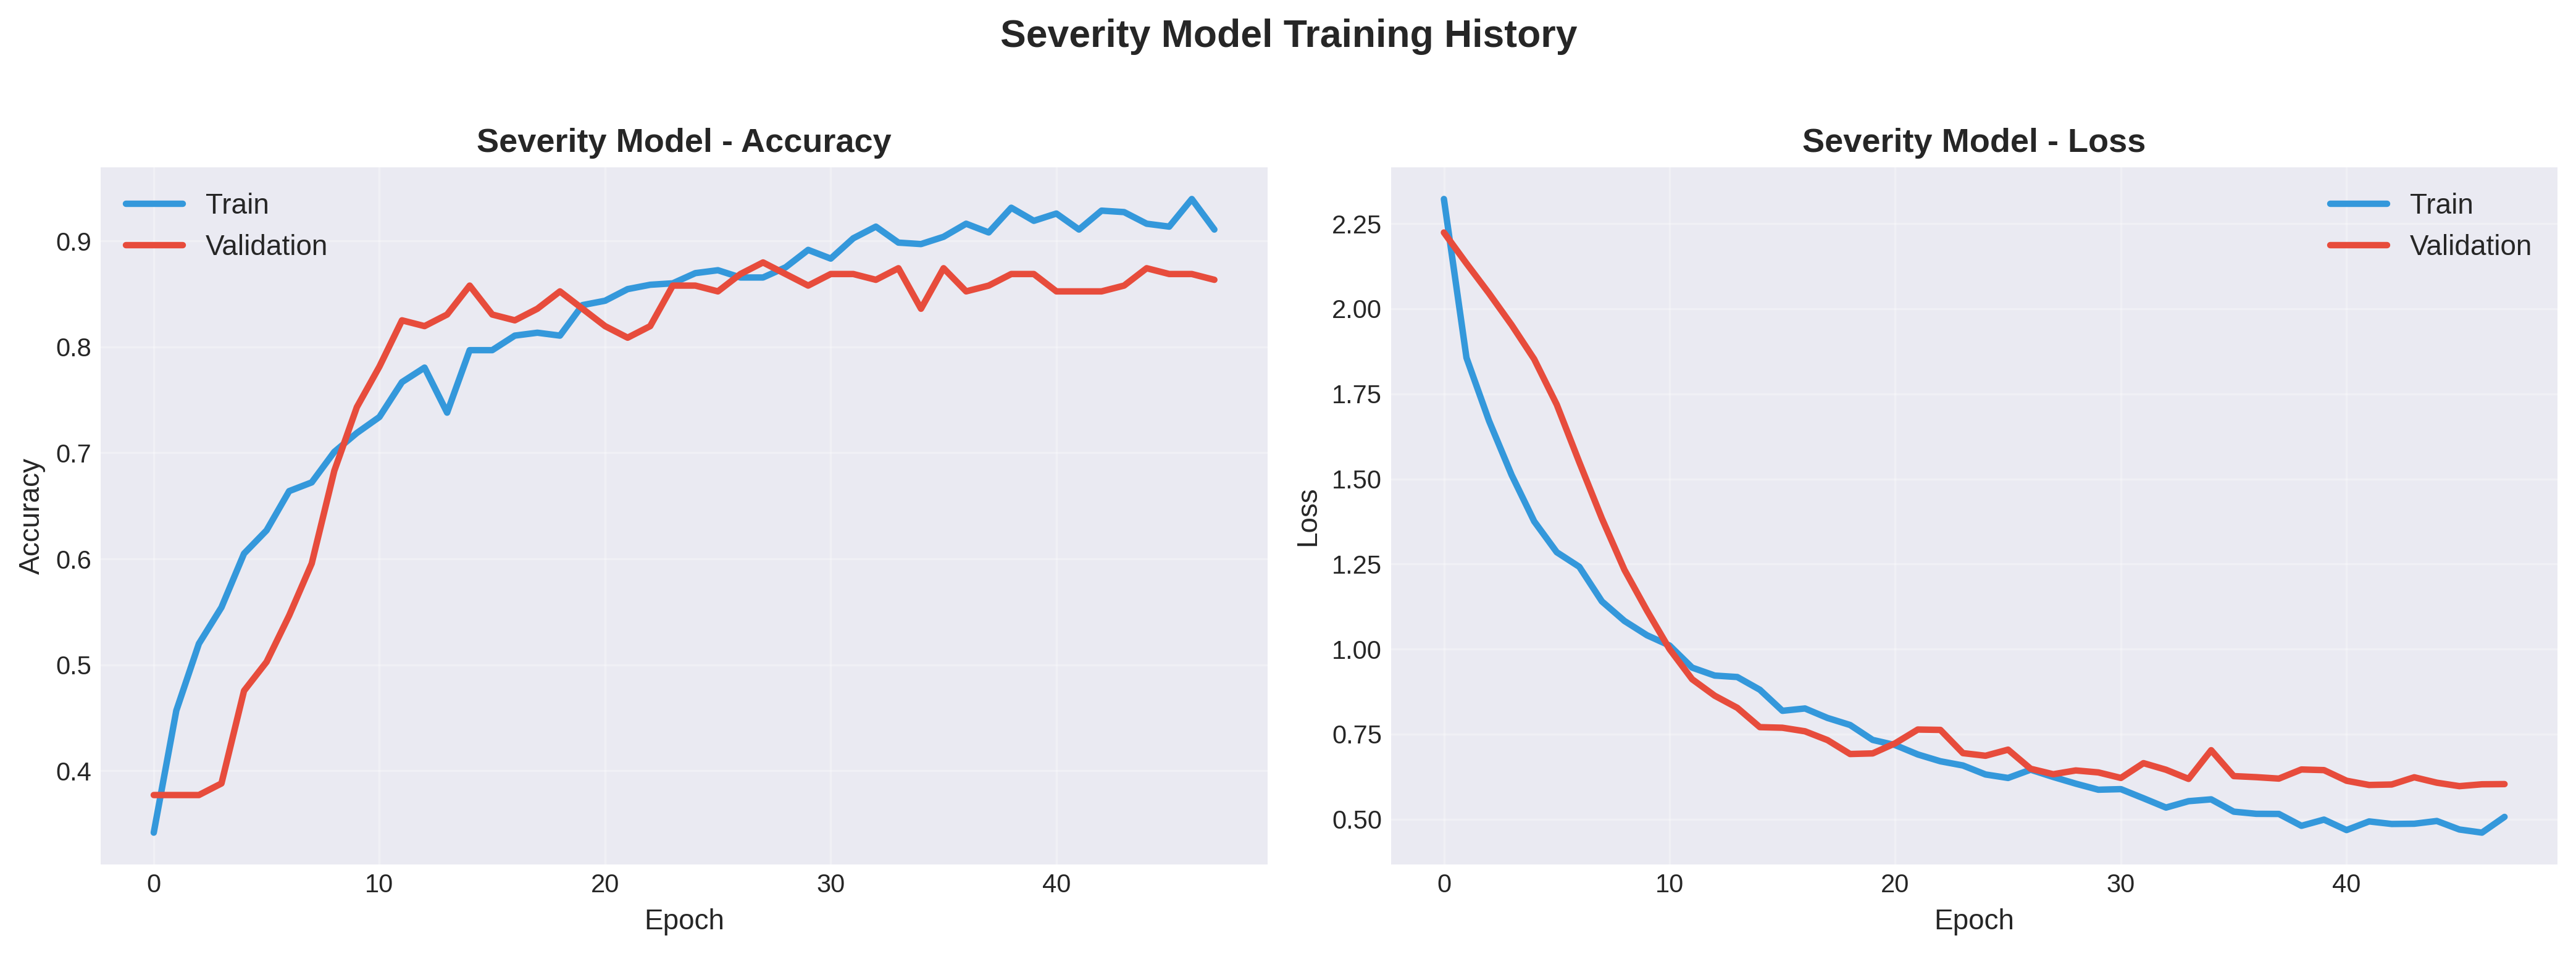
\includegraphics[width=0.85\columnwidth]{training_history.png}
    \caption{\textcolor{blue}{Bidirectional LSTM training history showing (left) accuracy convergence and (right) loss reduction over 50 epochs for severity prediction.}}
    \label{fig:training_history}
\end{figure}

\begin{figure}[ht!]
    \centering
    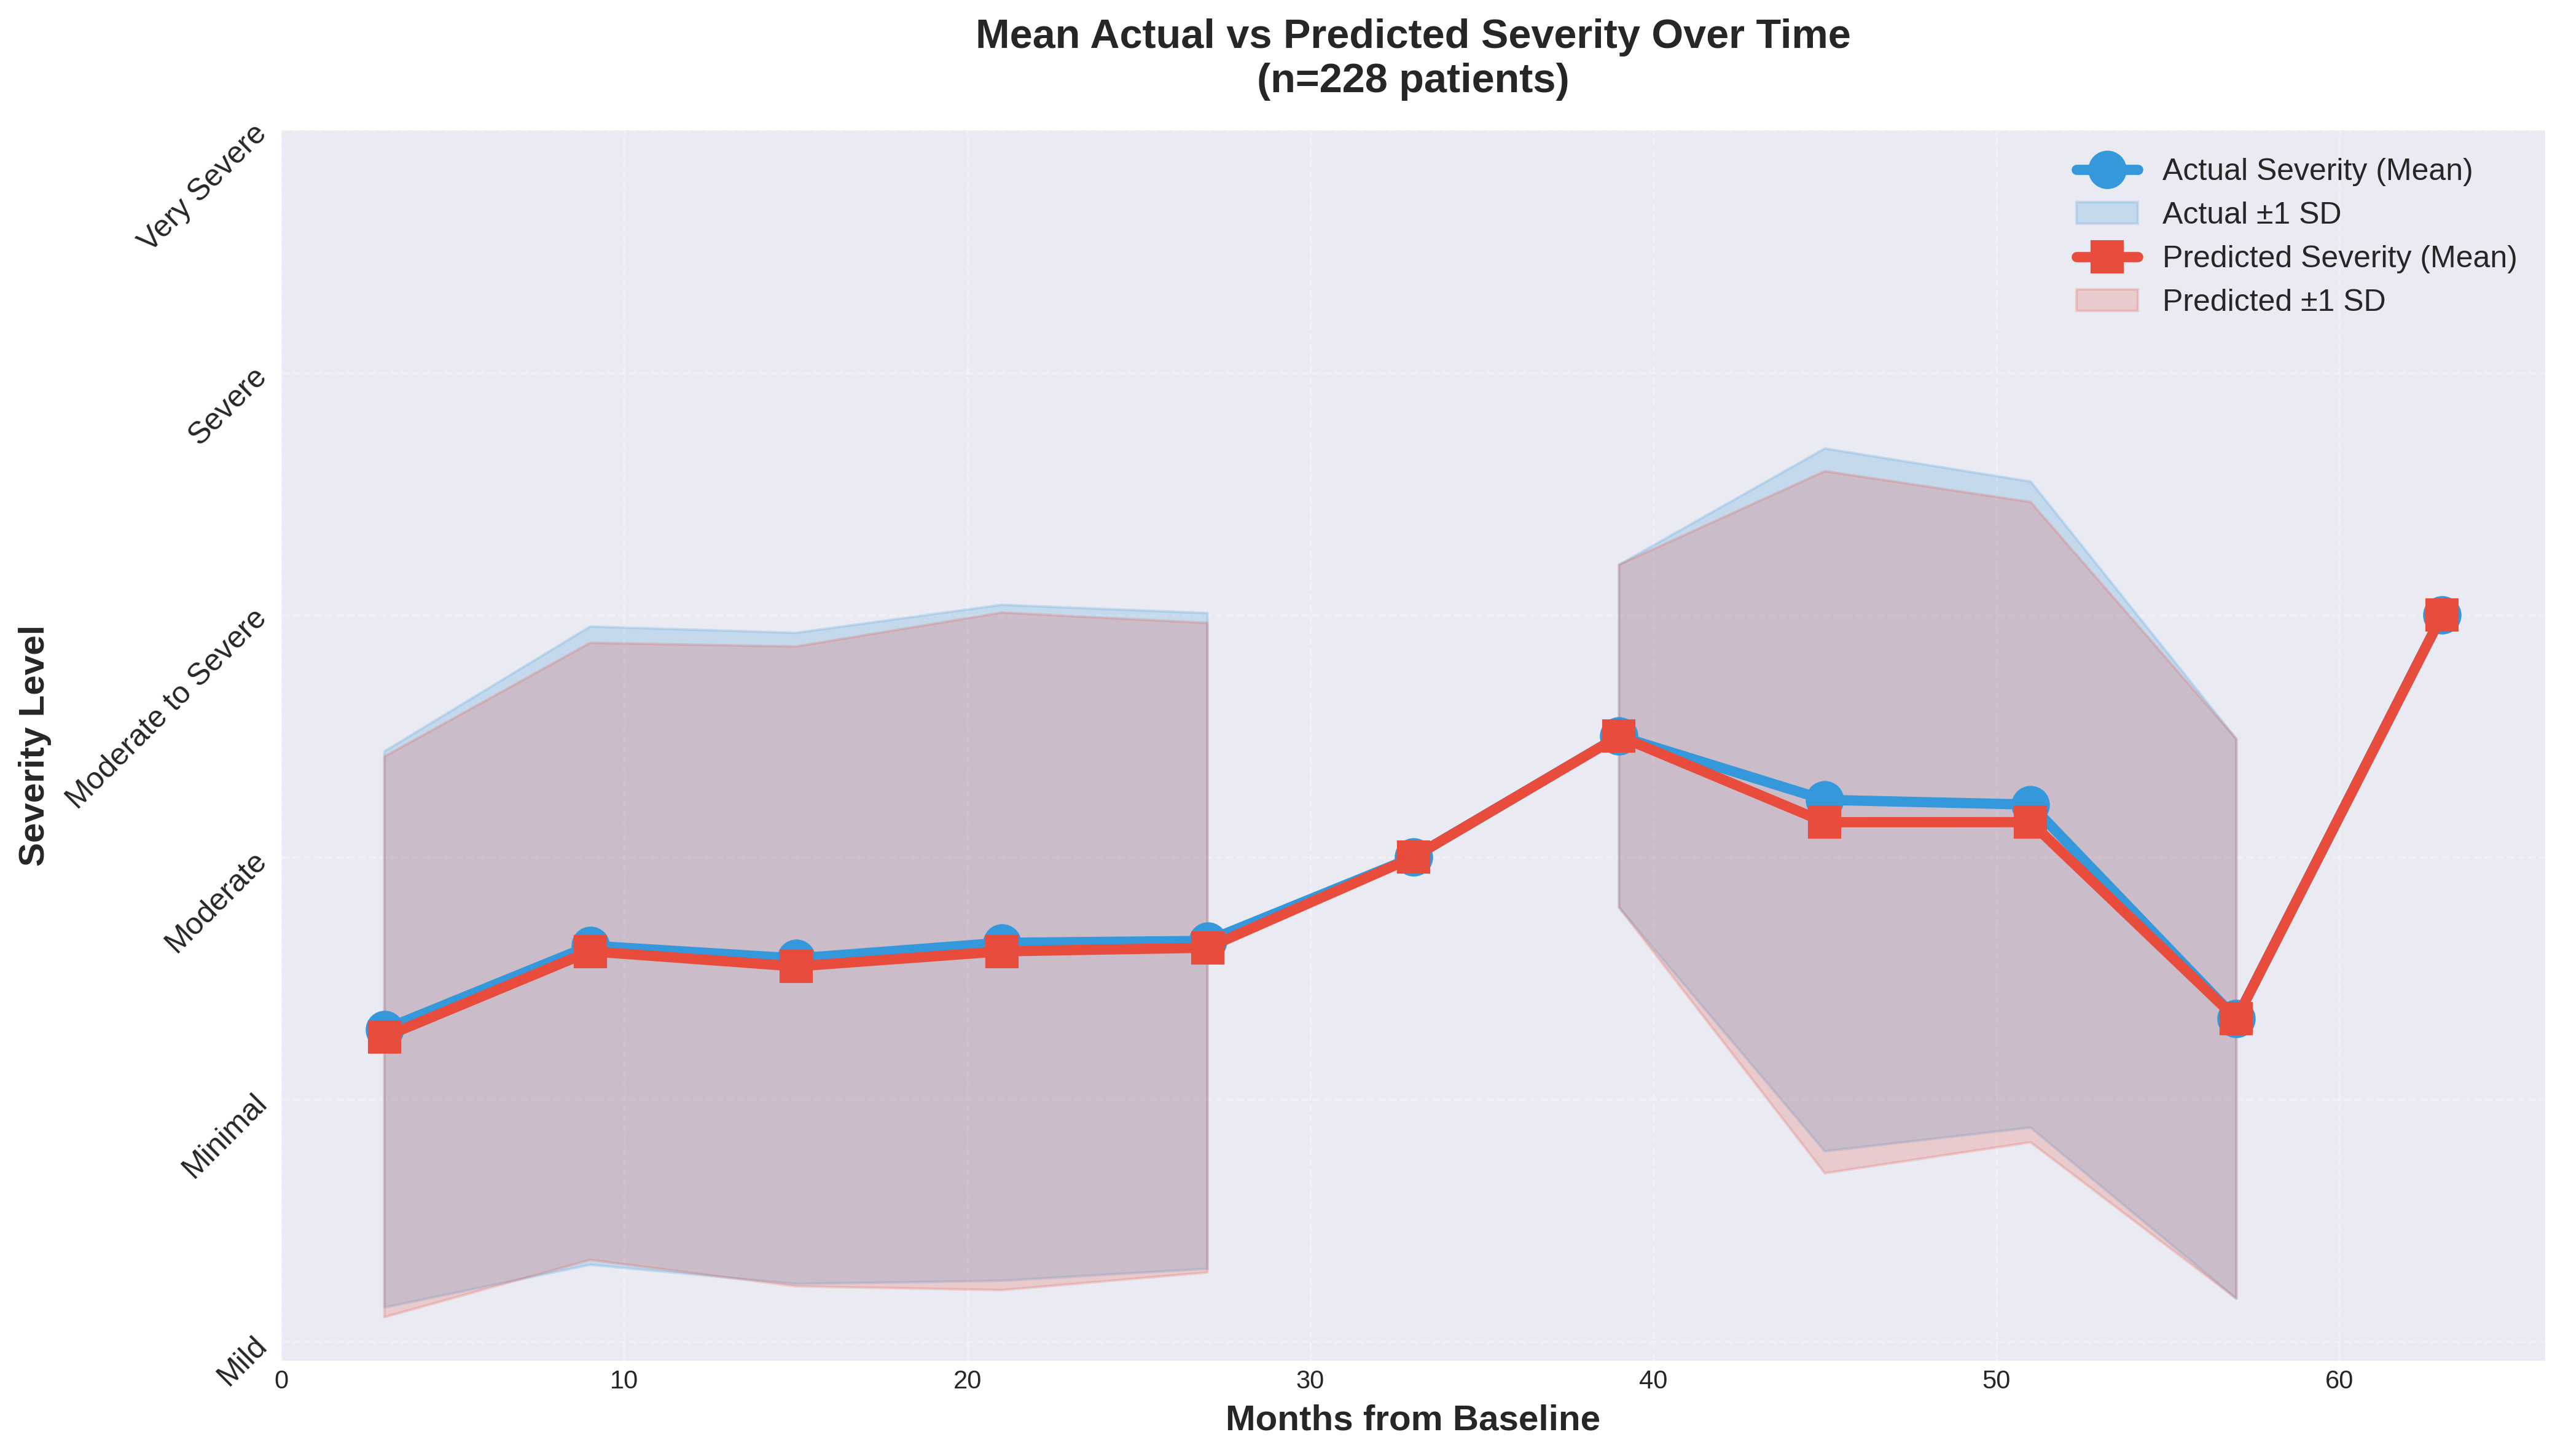
\includegraphics[width=0.85\columnwidth]{population_progression.png}
    \caption{\textcolor{blue}{Mean actual vs predicted severity progression over time across 228 PD patients. Shaded regions indicate ±1 standard deviation, demonstrating model's ability to capture population-level disease trajectory.}}
    \label{fig:population_progression}
\end{figure}

\begin{figure}[ht!]
    \centering
    \includegraphics[width=0.85\columnwidth]{patient_progression.png}
    \caption{\textcolor{blue}{Representative individual patient (ID: 3066) severity progression, showing precise alignment between actual and predicted severity levels across 60 months of follow-up.}}
    \label{fig:patient_progression}
\end{figure}


% ---------------------------------------------
\section{Discussion}
\label{Discussion}

Our proposed multilevel Parkinson's disease progression model shows its competence and dependability in assessing the progression of patients with PD from DaTscan radiomics data and clinical motor data. Although a diverse number of publications on the application of machine learning techniques to the diagnosis of PD have been published, most of the previous machine learning works in the diagnosis and assessment of PD were limited to the analysis of motor symptoms, kinematics, and wearable sensor data. In addition, most of them only used traditional machine learning algorithms to classify PD from healthy patients. In our work, we not only used expert-verified clinical motor data from PPMI, but also used DaTscan radiomics data of patients with PD, and used several ML and statistical-based approaches to aid our claim.

\subsection{Discussion on Hybrid Clinical and Imaging Dataset}
In our study, we introduce a hybrid dataset that combines clinical motor assessment data and radiomics-extracted features from DaTscan SPECT. Both datasets are obtained from the PPMI Database. 

The DaTscan radiomics data we obtained from the PPMI database did not have any segmentation mask, so we had to manually segment the images using a modified K-Means Clustering algorithm and acquire 25 necessary radiomics features from the caudate nucleus and putamen of the dorsal striatum region in the brain, which are our ROIs. On the other hand, we already had the MDS-UPDRS data from the same database from which we acquired the necessary 59 clinical motor data points. Together, these motor-based clinical and radiomics-extracted features help us to predict the progression of PD and the features that are highly responsible for the severity and progression of the disease. The 4 feature-ranking techniques provide all the topmost clinical features that are responsible for the progression of Parkinson's disease. The LDA gives us the best imaging features that are correlated with disease progression. Moreover, all the feature ranking techniques give us some common clinical features. 

The ANOVA and Kruskal-Wallis test were performed to validate the significance of the selected clinical feature. The ANOVA test at every visit gives a high F-statistic value and a low p-value $(p < 0.05)$ in brightness, standard deviation, mean, Gabor entropy, and skewness, which are radiomics-extracted features. The ANOVA test in disease severity also gives the same feature as statistical significance in disease progression analysis. The Kruskal-Wallis test in disease severity and patient visit also gives the same radiomics feature a high H-statistic and a low p-value. The ANOVA and Kruskal-Wallis test among the clinically ranked features give high F-statistic and H-statistic with a very low p-value for almost all features in the disease. 

The K-Means clustering technique and the agglomerative clustering both approaches demonstrated high scores for the Adjusted Rand Index (ARI) and Normalized Mutual Information (NMI). These results indicate that the underlying structure of the data is successfully captured by the LDA components, allowing the clustering at specific levels of severity of the disease and demonstrating that the data are well clustered in the LDA-reduced space (see Figure \ref{fig3}). This means that the progression of the disease and the severity stage can be determined by LDA. We compared the K-Means and Agglomerative clustering labels with the actual disease severity labels in Figure \ref{fig:fig5} and observed slight overlaps between the Mild and Minimal groups, the fifth and second clusters for Agglomerative Clustering, and the 0th and 5th clusters for K-Means. These overlaps highlight areas where further refinement in the clustering might be necessary. This phenomenon could be attributed to the early stages of Parkinson's disease, where symptoms often overlap between Minimal and Mild patients, making it challenging to distinguish these stages clearly in both clinical assessment and clustering outcomes. The probability density function (PDF) and the box plot of LD1 show a strong positive connection between the LD1 and LD2 scores and the degree of severity stage (see Figure \ref{fig:fig4}). LD1 values show a steadily rising trend with increasing severity, suggesting that higher scores correspond to more advanced stages of the disease, and the value of LD1 is distinct. These results highlight the possibility that LD1 can serve as a useful marker of the severity of the disease in individuals. For LD2, we observed that the correlation between the severity stage and LD2 is also positive, which means that the higher the value of LD2, the more severe the stage in which the patient is, except for the very severe stage. For the very severe stage, the value of LD2 is less than -5, and the value of LD2 for other stages of the disease is greater than -5.

Our findings in this study present significant insight into the relationship between clinical and radiomics-extracted features with PD severity and progression. In general, our analysis emphasizes the advantage of integrating clinical and imaging characteristics for a more robust assessment of PD.


\subsection{Discussion on Parkinson’s disease progression}

The progression analysis in this study provides a robust evaluation of Parkinson's disease progression by integrating both clinical motor assessment and DaTscan SPECT imaging biomarkers.

By examining progression across disease severity (see Table \ref{tab:tab8}) and patient visits (see Table \ref{tab:tab9}), and by identifying key features influencing progression (see Table \ref{tab:key_clinical_imaging_features}), our findings offer robust insights into the mixed nature of PD decline.
Table \ref{tab:tab8} clarifies the distinct vulnerability of clinical and imaging variables. 30 Clinical features ranked by the four ranking techniques show high progression during the early transition, for example, 73.33\% progression between Minimal vs Mild stages, and a significant increase to 100\% and 96.67\% between Minimal vs Severe stage and Minimal vs Very Severe stage. Between the Severe vs Very Severe stage, almost 67.67\% clinical biomarkers show progression. On the contrary, SPECT imaging markers express more moderate changes in the early stages, for example, 13.64\% in the Minimal vs Mild stage, and gradually increase in progressive shifts up to 54.55\%, where the shift between Severe vs Very Severe stage gives 36.36\% progression. The progression percentages fall into an intermediate but more balanced range (48–78.84\%) when these two data modalities are assembled into a single set of 52 characteristics. We can notice a significant progression between every disease stage. Both the modest early functional changes and the more noticeable neurodegenerative abnormalities visible in later stages are captured by this integrated method, which successfully overcomes the inherent disparities between functional and structural evaluations.

Through longitudinal analysis, Table \ref{tab:tab9} supports even more the value of a multi-modal strategy. Although short-term intervals (e.g., between Visit 1 and Visit 2) provide somewhat reduced progression rates of 33.30\%, 36.36\%, and 34.60\% across clinical features, imaging features, and combined hybrid features analysis, longer intervals (e.g., between Visit 1 and Visit 4) reveal a clear rise in progression. Specifically, the clinical characteristics of MDS-UPDRS show an 83.30\% advancement, while the combined dataset shows a notable 67.30\% change, exceeding the separate imaging features, which reach just 45.50\%. 

These findings show that when clinical symptoms and imaging indicators are coupled, temporal changes in Parkinson's disease can be more accurately reported. This shows that an integrated framework is required to follow the disease's course throughout time accurately. Additionally, we can see that Parkinson's disease develops slowly in the beginning and progressively worsens with time. Given the aggressive progression of PD severity, prodromal or early-stage PD cohorts-even those with minimal baseline impairment-require systematic clinical reassessment regularly to mitigate rapid neurodegeneration.

% Analyzing disease progression revealed a significant degree of variability in PD characteristics, with distinct shifts in both motor and non-motor features observed across severity from early, minimal phases to advanced, severe stages. Likewise, we encountered a similar presentation across visits showing significant differences from the first visit to the fourth visit. 

When we align the significant features with real-world activities, in Table \ref{tab:key_clinical_imaging_features}, we identify the key functional impairments that PD patients face in their daily lives. It includes dressing (NP2DRES) and getting out of bed, a car, or a deep chair (NP2RISE), which is common in both disease severity and visits, drawing attention to its importance. NP2DRES gave an ANOVA score (F statistic: 107.61, p-value: 3.26E-89) and a Kruskal-Wallis score (H statistic: 313.693, p-value: 1.14E-65) for the severity of the disease and an ANOVA score (14.984, 1.59E-09) and a Kruskal-Wallis score (40.805, 7.19E-09) for visits. Similarly, NP2RISE gave an ANOVA score (82.652, 1.51E-71) and a Kruskal-Wallis score (245.612, 4.80E-51) with respect to disease severity, and an ANOVA score (12.921, 2.86E-08) and a Kruskal-Wallis score (32.564, 3.98E-07) in visits. 

Furthermore, strong statistical analysis in section \ref{PD Progression Result} provided that PD individuals have difficulty performing other daily activities such as hobbies (NP2HOBB), eating tasks (NP2EAT), turning on bed (NP2TURN), and walking or balance impairments (NP2WALK), along with daytime sleepiness (NP1SLPD). Patients may also experience reduced global spontaneity of movement (NP3BRADY), impaired posture (NP3POSTR), and face challenges that arise from a chair (NP3RISNG). The progression of key imaging features such as Gabor Energy (capturing edge and texture information), Brightness (average intensity of pixels), Mean (Mean pixel intensity), etc., established in our study, was correlated with the subsequent stages of disease severity, as observed during sequential clinical visits, highlighting their diagnostic relevance in DaTscan SPECT data.


\textcolor{blue}{
\subsection{Longitudinal modeling for personalized disease monitoring}
With an AUC of 0.9814 and a test accuracy of 87.98\% (95\% CI: 85.1-90.3\%), the bidirectional LSTM model showed exceptional discriminative performance across all six severity classes.   The model showed low overfitting even after processing 228 patients over four consecutive timepoints (baseline, 12, 24, and 48 months), with training accuracy of 95.34\% and validation accuracy of 85.25\%.   Balanced precision (86.72\%) and recall (87.98\%) measures validate consistent performance across severity categories with an F1-score of 87.15\%. Training dynamics (Figure \ref{fig:training_history}) demonstrate consistent convergence over 50 epochs, with accuracy curves continuously increasing and loss curves constantly declining.  The model's ability to generalize to unknown temporal sequences is confirmed by the strong agreement between training and validation metrics.  With standard deviation regions reflecting inherent inter-patient variability in disease progression rates, population-level trajectory analysis (Figure \ref{fig:population_progression}) shows that the model was able to capture mean severity progression across 228 patients over the course of the 60-month observation period.  Individualized severity predictions that take temporal dynamics into account are made possible by the bidirectional architecture's successful capture of both prospective trajectory patterns and retrospective patient history. A detailed alignment between anticipated and actual severity transitions is demonstrated by the individual patient analysis (Figure \ref{fig:patient_progression}).  The model's clinical usefulness for individualized monitoring is demonstrated by Patient 3066's progression from Minimal severity at baseline to Moderate-to-Severe at 48 months.  By integrating 84 multimodal features across successive timepoints, the attention mechanism makes it possible to identify patients who may be at risk of accelerated progression, allowing for prompt clinical interventions and the development of optimal treatment plans.  Beyond traditional cross-sectional evaluations, this longitudinal framework gives physicians a quantitative tool for monitoring the progression of diseases.
}
\subsection{Limitation and Future Scope}
While working with the data provided by the Parkinson's progression markers initiative, we encountered a few problems. One problem was that not all patients had DaTscan radiomics data, and because of that, even though we had more samples in the MDS-UPDRS clinical data, we had to work with only 228 patients.
%Some patients had multiple visits in one year, and some did not continue after one or two sessions. Furthermore, we previously mentioned that the DaTscan radiomicss had missing segmentation masks, which, if they exist, could help us to do the segmentation more efficiently. The motor assessment data also had some missing and invalid values.
In the future, we want to use MRI scans together with DaTscan to improve the performance of our model. In this work, we only used the motor assessment data for our analysis, but we also have access to the non-motor assessment of PPMI, medical history, subject characteristics, and genetic data, which we plan to use in our future work.


% ---------------------------------------------
\section{Conclusion}
\label{Conclusion}

Our study proposes a novel approach to diagnose and monitor the progression of Parkinson's disease in four visits and at different levels of severity of the disease, utilizing both DaTscan SPECT imaging and clinical data from the MDS-UPDRS scale. We created a Radiomics-MDS-UPDRS dataset that significantly improved classification accuracy using advanced segmentation and feature extraction techniques. The use of Linear Discriminant Analysis highlighted key DaTscan SPECT imaging features, which are essential to differentiate the severity of Parkinson's disease into six categories. Furthermore, our progression analysis revealed valuable insights into how disease severity changes over time, very effectively by analyzing both severity progression and the patients' progression of Parkinson's disease during visits. In addition, this study aims to improve diagnostic precision by proposing a new progression analysis system, making it a valuable tool for clinical applications in the care of Parkinson's disease.


\section*{Declarations}
\noindent
\textbf{Ethics approval and consent to participate:} Not applicable. \\
\textbf{Data availability:}  We use the publicly available Parkinson's Progression Markers Initiative (PPMI) \cite{marek2011parkinson} dataset. Additionally, we created a dataset, Radiomics-MDS-UPDRS. In our dataset, the Radiomics data will be made available on a reasonable request for non-commercial academic purposes. Access to the complete Radiomics-MDS-UPDRS dataset requires a proof of authorization from the International Parkinson and Movement Disorder Society (MDS), which can be obtained from
\href{https://mds.movementdisorders.org/publications/rating_scales/request_form.php}{here}.  The use of the dataset for commercial purposes is not allowed. \\
\textbf{Conflict of interest/Competing interests:} The authors declare that they have no financial conflicts of interest or personal relationships that could have influenced this work.\\
\textbf{Funding:} This study does not include any external funding.

\begin{thebibliography}{10}
\setlength{\itemsep}{0.2em}
\setlength{\parskip}{0pt}
\providecommand{\url}[1]{#1}
\csname url@samestyle\endcsname
\providecommand{\newblock}{\relax}
\providecommand{\bibinfo}[2]{#2}
\providecommand{\BIBentrySTDinterwordspacing}{\spaceskip=0pt\relax}
\providecommand{\BIBentryALTinterwordstretchfactor}{4}
\providecommand{\BIBentryALTinterwordspacing}{\spaceskip=\fontdimen2\font plus
\BIBentryALTinterwordstretchfactor\fontdimen3\font minus
  \fontdimen4\font\relax}
\providecommand{\BIBforeignlanguage}[2]{{%
\expandafter\ifx\csname l@#1\endcsname\relax
\typeout{** WARNING: IEEEtran.bst: No hyphenation pattern has been}%
\typeout{** loaded for the language `#1'. Using the pattern for}%
\typeout{** the default language instead.}%
\else
\language=\csname l@#1\endcsname
\fi
#2}}
\providecommand{\BIBdecl}{\relax}
\BIBdecl

\bibitem{DBLP:journals/fgcs/AbdulhayNNVV18}
E.~Abdulhay, N.~Arunkumar, K.~Narasimhan, E.~Vellaiappan, and V.~Venkatraman,
``Gait and tremor investigation using machine learning techniques for the diagnosis of Parkinson disease,''
\emph{Future Generation Computer Systems}, vol.~83, pp.~366--373, 2018.

\bibitem{lundervold2019overview}
A.~S. Lundervold and A.~Lundervold, ``An overview of deep learning in medical
  imaging focusing on mri,'' \emph{Zeitschrift f{\"u}r Medizinische Physik},
  vol.~29, no.~2, pp. 102--127, 2019.

\bibitem{majhi2024improved}
B.~Majhi, A.~Kashyap, S.~S. Mohanty, S.~Dash, S.~Mallik, A.~Li, and Z.~Zhao,
  ``An improved method for diagnosis of parkinson’s disease using deep
  learning models enhanced with metaheuristic algorithm,'' \emph{BMC medical
  imaging}, vol.~24, no.~1, p. 156, 2024.

\bibitem{hirschauer2015computer}
T.~J. Hirschauer, H.~Adeli, and J.~A. Buford, ``Computer-aided diagnosis of
  parkinson’s disease using enhanced probabilistic neural network,''
  \emph{Journal of medical systems}, vol.~39, pp. 1--12, 2015.

\bibitem{suwijn2015diagnostic}
S.~R. Suwijn, C.~J. van Boheemen, R.~J. de~Haan, G.~Tissingh, J.~Booij, and
  R.~M. de~Bie, ``The diagnostic accuracy of dopamine transporter spect imaging
  to detect nigrostriatal cell loss in patients with parkinson’s disease or
  clinically uncertain parkinsonism: a systematic review,'' \emph{EJNMMI
  research}, vol.~5, pp. 1--8, 2015.

\bibitem{adeli2017kernel}
E.~Adeli, G.~Wu, B.~Saghafi, L.~An, F.~Shi, and D.~Shen, ``Kernel-based joint
  feature selection and max-margin classification for early diagnosis of
  parkinson’s disease,'' \emph{Scientific reports}, vol.~7, no.~1, p. 41069,
  2017.

\bibitem{khachnaoui2020machine}
H.~Khachnaoui, R.~Mabrouk, and N.~Khlifa, ``Machine learning and deep learning
  for clinical data and pet/spect imaging in parkinson's disease: a review,''
  \emph{IET Image Processing}, vol.~14, no.~16, pp. 4013--4026, 2020.

\bibitem{chen2023detection}
B.~Chen, M.~Xu, H.~Yu, J.~He, Y.~Li, D.~Song, and G.~G. Fan, ``Detection of
  mild cognitive impairment in parkinson’s disease using gradient boosting
  decision tree models based on multilevel dti indices,'' \emph{Journal of
  Translational Medicine}, vol.~21, no.~1, p. 310, 2023.

\bibitem{booth2022predicting}
S.~Booth, K.~W. Park, C.~S. Lee, J.~H. Ko \emph{et~al.}, ``Predicting cognitive
  decline in parkinson’s disease using fdg-pet--based supervised learning,''
  \emph{The Journal of Clinical Investigation}, vol. 132, no.~20, 2022.

\bibitem{fiorenzato2024brain}
E.~Fiorenzato, S.~Moaveninejad, L.~Weis, R.~Biundo, A.~Antonini, and
  C.~Porcaro, ``Brain dynamics complexity as a signature of cognitive decline
  in parkinson's disease,'' \emph{Movement Disorders}, vol.~39, no.~2, pp.
  305--317, 2024.

\bibitem{amboni2022machine}
M.~Amboni, C.~Ricciardi, S.~Adamo, E.~Nicolai, A.~Volzone, R.~Erro, S.~Cuoco,
  G.~Cesarelli, L.~Basso, G.~D'Addio \emph{et~al.}, ``Machine learning can
  predict mild cognitive impairment in parkinson's disease,'' \emph{Frontiers
  in neurology}, vol.~13, p. 1010147, 2022.

\bibitem{amoroso2018complex}
N.~Amoroso, M.~La~Rocca, A.~Monaco, R.~Bellotti, and S.~Tangaro, ``Complex
  networks reveal early mri markers of parkinson’s disease,'' \emph{Medical
  image analysis}, vol.~48, pp. 12--24, 2018.

\bibitem{khachnaoui2023enhanced}
H.~Khachnaoui, B.~Chikhaoui, N.~Khlifa, and R.~Mabrouk, ``Enhanced
  parkinson’s disease diagnosis through convolutional neural network models
  applied to spect datscan images,'' \emph{IEEE Access}, 2023.

\bibitem{hsu2020classification}
S.-Y. Hsu, L.-R. Yeh, T.-B. Chen, W.-C. Du, Y.-H. Huang, W.-H. Twan, M.-C. Lin,
  Y.-H. Hsu, Y.-C. Wu, and H.-Y. Chen, ``Classification of the multiple stages
  of parkinson’s disease by a deep convolution neural network based on
  99mtc-trodat-1 spect images,'' \emph{Molecules}, vol.~25, no.~20, p. 4792,
  2020.

\bibitem{magesh2020explainable}
P.~R. Magesh, R.~D. Myloth, and R.~J. Tom, ``An explainable machine learning
  model for early detection of parkinson's disease using lime on datscan
  imagery,'' \emph{Computers in Biology and Medicine}, vol. 126, p. 104041,
  2020.

\bibitem{hathaliya2022convolutional}
J.~Hathaliya, R.~Parekh, N.~Patel, R.~Gupta, S.~Tanwar, F.~Alqahtani,
  M.~Elghatwary, O.~Ivanov, M.~S. Raboaca, and B.-C. Neagu, ``Convolutional
  neural network-based parkinson disease classification using spect imaging
  data,'' \emph{Mathematics}, vol.~10, no.~15, p. 2566, 2022.

\bibitem{reyes2019lstm}
J.~F.~Reyes, J.~S.~Montealegre, Y.~J.~Castano, C.~Urcuqui, and A.~Navarro,
``LSTM and convolution networks exploration for Parkinson’s diagnosis,''
in \emph{Proceedings of the 2019 IEEE Colombian Conference on Communications and Computing (COLCOM)}, 
pp.~1--4, 2019.

\bibitem{DBLP:conf/bibm/YagisHC19}
E.~Yagis, A.~G.~S.~De~Herrera, and L.~Citi,
``Generalization performance of deep learning models in neurodegenerative disease classification,''
in \emph{Proceedings of the 2019 IEEE International Conference on Bioinformatics and Biomedicine (BIBM)}, 
pp.~1692--1698, 2019.

\bibitem{ali2019multi}
L.~Ali, S.~U.~Khan, M.~Arshad, S.~Ali, and M.~Anwar,
``A multi-model framework for evaluating type of speech samples having complementary information about Parkinson's disease,''
in \emph{Proceedings of the 2019 International Conference on Electrical, Communication, and Computer Engineering (ICECCE)}, 
pp.~1--5, 2019.

\bibitem{martinez2018kinematic}
M.~Mart{\'\i}nez, F.~Villagra, J.~M. Castellote, and M.~A. Pastor, ``Kinematic
  and kinetic patterns related to free-walking in parkinson’s disease,''
  \emph{Sensors}, vol.~18, no.~12, p. 4224, 2018.

\bibitem{adeli2018semi}
E.~Adeli, K.-H. Thung, L.~An, G.~Wu, F.~Shi, T.~Wang, and D.~Shen,
  ``Semi-supervised discriminative classification robust to sample-outliers and
  feature-noises,'' \emph{IEEE transactions on pattern analysis and machine
  intelligence}, vol.~41, no.~2, pp. 515--522, 2018.

\bibitem{DBLP:journals/ijmi/PrashanthRMG16}
R.~Prashanth, S.~D.~Roy, P.~K.~Mandal, and S.~Ghosh,
``High-accuracy detection of early Parkinson's disease through multimodal features and machine learning,''
\emph{International Journal of Medical Informatics}, vol.~90, pp.~13--21, 2016.

\bibitem{hajianfar2023prediction}
G.~Hajianfar, S.~Kalayinia, M.~Hosseinzadeh, S.~Samanian, M.~Maleki, V.~Sossi,
  A.~Rahmim, and M.~R. Salmanpour, ``Prediction of parkinson’s disease
  pathogenic variants using hybrid machine learning systems and radiomic
  features,'' \emph{Physica Medica}, vol. 113, p. 102647, 2023.

\bibitem{harvey2022machine}
J.~Harvey, R.~A.~Reijnders, R.~Cavill, A.~Duits, S.~K{\"o}hler, L.~Eijssen, B.~P.~F.~Rutten, \emph{et~al.},
``Machine learning-based prediction of cognitive outcomes in de novo Parkinson’s disease,''
\emph{npj Parkinson's Disease}, vol.~8, no.~1, p.~150, 2022.

\bibitem{DBLP:journals/tnn/HuangLCFXEQL22}
Z.~Huang, H.~Lei, G.~Chen, A.~F.~Frangi, Y.~Xu, A.~Elazab, J.~Qin, and B.~Lei,
``Parkinson’s disease classification and clinical score regression via united embedding and sparse learning from longitudinal data,''
\emph{IEEE Transactions on Neural Networks and Learning Systems}, vol.~33, no.~8, pp.~3357--3371, 2021.

\bibitem{prashanth2018early}
R.~Prashanth and S.~D. Roy, ``Early detection of parkinson’s disease through
  patient questionnaire and predictive modelling,'' \emph{International journal
  of medical informatics}, vol. 119, pp. 75--87, 2018.

\bibitem{ali2019reliable}
L.~Ali, C.~Zhu, N.~A.~Golilarz, A.~Javeed, M.~Zhou, and Y.~Liu,
``Reliable Parkinson’s disease detection by analyzing handwritten drawings: construction of an unbiased cascaded learning system based on feature selection and adaptive boosting model,''
\emph{IEEE Access}, vol.~7, pp.~116480--116489, 2019.

\bibitem{castillo2018robust}
D.~Castillo-Barnes, J.~Ram{\'\i}rez, F.~Segovia, F.~J. Mart{\'\i}nez-Murcia,
  D.~Salas-Gonzalez, and J.~M. G{\'o}rriz, ``Robust ensemble classification
  methodology for i123-ioflupane spect images and multiple heterogeneous
  biomarkers in the diagnosis of parkinson's disease,'' \emph{Frontiers in
  Neuroinformatics}, vol.~12, p.~53, 2018.

\bibitem{ahmadi2019towards}
S.-A. Ahmadi, G.~Vivar, J.~Frei, S.~Nowoshilow, S.~Bardins, T.~Brandt, and
  S.~Krafczyk, ``Towards computerized diagnosis of neurological stance
  disorders: data mining and machine learning of posturography and sway,''
  \emph{Journal of Neurology}, vol. 266, pp. 108--117, 2019.

\bibitem{buongiorno2019low}
D.~Buongiorno, I.~Bortone, G.~D. Cascarano, G.~F. Trotta, A.~Brunetti, and
  V.~Bevilacqua, ``A low-cost vision system based on the analysis of motor
  features for recognition and severity rating of parkinson’s disease,''
  \emph{BMC Medical Informatics and Decision Making}, vol.~19, pp. 1--13, 2019.

\bibitem{cavallo2019upper}
F.~Cavallo, A.~Moschetti, D.~Esposito, C.~Maremmani, and E.~Rovini, ``Upper
  limb motor pre-clinical assessment in parkinson's disease using machine
  learning,'' \emph{Parkinsonism \& related disorders}, vol.~63, pp. 111--116,
  2019.

\bibitem{zhang2023multi}
X.~Zhang, Y.~Zhou, Z.~Lu, D.~Zhai, H.~Luo, T.~Li, and Y.~Li, ``Multi-level
  graph neural network with sparsity pooling for recognizing parkinson’s
  disease,'' \emph{IEEE Transactions on Neural Systems and Rehabilitation
  Engineering}, 2023.

\bibitem{DBLP:conf/amia/Zhang00LZW18}
X.~Zhang, L.~He, K.~Chen, Y.~Luo, J.~Zhou, and F.~Wang,
``Multi-view graph convolutional network and its applications on neuroimage analysis for Parkinson’s disease,''
in \emph{Proceedings of the AMIA Annual Symposium}, vol.~2018, p.~1147, 2018.

\bibitem{marek2011parkinson}
K.~Marek, D.~Jennings, S.~Lasch, A.~Siderowf, C.~Tanner, T.~Simuni, C.~Coffey,
  K.~Kieburtz, E.~Flagg, S.~Chowdhury \emph{et~al.}, ``The parkinson
  progression marker initiative (ppmi),'' \emph{Progress in neurobiology},
  vol.~95, no.~4, pp. 629--635, 2011.

\bibitem{ali2014kruskal}
S.~Ali~Khan, A.~Hussain, A.~Basit, and S.~Akram, ``Kruskal-wallis-based
  computationally efficient feature selection for face recognition,'' \emph{The
  Scientific World Journal}, vol. 2014, no.~1, p. 672630, 2014.

\bibitem{mercer2024practical}
M.~K. Mercer, J.~W. Revels, L.~C. Blacklock, K.~P. Banks, L.~S. Johnson, D.~H. Lewis, P.~H. Kuo, S.~Wilson, S.~Elojeimy, ``Practical Overview of 123I-Ioflupane Imaging in Parkinsonian Syndromes,'' \emph{RadioGraphics}, vol.~44, no.~2, pp. e230133, 2024.

\bibitem{morbelli2020eanm}
S.~Morbelli, G.~Esposito, J.~Arbizu, H.~Barthel, R.~Boellaard, N.~I. Bohnen, D.~J. Brooks, J.~Darcourt, J.~C. Dickson, D.~Douglas \emph{et~al.}, ``EANM practice guideline/SNMMI procedure standard for dopaminergic imaging in Parkinsonian syndromes 1.0,'' \emph{European journal of nuclear medicine and molecular imaging}, vol.~47, no.~8, pp. 1885--1912, 2020.

\bibitem{mayerhoefer2020introduction}
M.~E. Mayerhoefer, A.~Materka, G.~Langs, I.~H{\"a}ggstr{\"o}m, P.~Szczypi{\'n}ski, P.~Gibbs, G.~Cook, ``Introduction to radiomics,'' \emph{Journal of Nuclear Medicine}, vol.~61, no.~4, pp. 488--495, 2020.

\end{thebibliography}

\end{document}